%%%%%%%%%%%%%%%%%%%%%%%%%%%%%%%%%%%%%%%%%
% Oliver Lemon made minor edits (jan 2015)  to : 
% Masters/Doctoral Thesis 
% LaTeX Template
% Version 1.43 (17/5/14)
%
% This template has been downloaded from:
% http://www.LaTeXTemplates.com
%
% Original authors:
% Steven Gunn 
% http://users.ecs.soton.ac.uk/srg/softwaretools/document/templates/
% and
% Sunil Patel
% http://www.sunilpatel.co.uk/thesis-template/
%
% License:
% CC BY-NC-SA 3.0 (http://creativecommons.org/licenses/by-nc-sa/3.0/)
%
% Note:
% Make sure to edit document variables in the Thesis.cls file
%
%%%%%%%%%%%%%%%%%%%%%%%%%%%%%%%%%%%%%%%%%

%----------------------------------------------------------------------------------------
%	PACKAGES AND OTHER DOCUMENT CONFIGURATIONS
%----------------------------------------------------------------------------------------

\documentclass[11pt, oneside]{Thesis} % The default font size and one-sided printing (no margin offsets)

\graphicspath{{Pictures/}} % Specifies the directory where pictures are stored
\usepackage{subfig}
\usepackage[square, comma, sort&compress, numbers]{natbib} % Use the natbib reference package - read up on this to edit the reference style; if you want text (e.g. Smith et al., 2012) for the in-text references (instead of numbers), remove 'numbers' 
% Added by me
\hypersetup{pdfencoding=auto,psdextra, urlcolor=blue, linkcolor=red, citecolor=blue,  colorlinks=true} % Colors hyperlinks in blue - change to black if annoying
\usepackage{comment
}
\usepackage{amsfonts}
\usepackage{booktabs}
\usepackage{siunitx}

\usepackage{cleveref}
\crefname{section}{§}{§§}
\Crefname{section}{§}{§§}

\title{HWU CS Masters thesis template} % BUT you should use use " \title{\ttitle} " here instead to define the thesis title ! 
% \ttitle is defined in the file Thesis.cls 

\begin{document}

\frontmatter % Use roman page numbering style (i, ii, iii, iv...) for the pre-content pages

\setstretch{1.3} % Line spacing of 1.3

% Define the page headers using the FancyHdr package and set up for one-sided printing
\fancyhead{} % Clears all page headers and footers
\rhead{\thepage} % Sets the right side header to show the page number
\lhead{} % Clears the left side page header

\pagestyle{fancy} % Finally, use the "fancy" page style to implement the FancyHdr headers

\newcommand{\HRule}{\rule{\linewidth}{0.5mm}} % New command to make the lines in the title page

% PDF meta-data
\hypersetup{pdftitle={\ttitle}}
\hypersetup{pdfsubject=\subjectname}
\hypersetup{pdfauthor=\authornames}
\hypersetup{pdfkeywords=\keywordnames}

%----------------------------------------------------------------------------------------
%	TITLE PAGE
%----------------------------------------------------------------------------------------

\begin{titlepage}
\begin{center}

\textsc{\LARGE \univname}\\[1.5cm] % University name
\textsc{\Large Masters Thesis}\\[0.5cm] % Thesis type

\HRule \\[0.4cm] % Horizontal line
{\huge \bfseries \ttitle}\\[0.4cm] % Thesis title
\HRule \\[1.5cm] % Horizontal line
 
\begin{minipage}{0.4\textwidth}
\begin{flushleft} \large
\emph{Author:}\\
{\authornames} % Author name - remove the \href bracket to remove the link
\end{flushleft}
\end{minipage}
\begin{minipage}{0.4\textwidth}
\begin{flushright} \large
\emph{Supervisor:} \\
{\supname} % Supervisor name - remove the \href bracket to remove the link  
\end{flushright}
\end{minipage}\\[3cm]
 
\large \textit{A thesis submitted in fulfilment of the requirements\\ for the degree of \degreename}\\[0.3cm] % University requirement text
\textit{in the}\\[0.4cm]
\groupname\\

\deptname\\[2cm] % Research group name and department name
 
{\large \today}\\[1cm] % Date

\includegraphics[width=4.0cm]{./Figures/UCTLogo.jpg} % University/department logo - uncomment to place it
 
\vfill
\end{center}

\end{titlepage}

%----------------------------------------------------------------------------------------
%	DECLARATION PAGE
%	Your institution may give you a different text to place here
%----------------------------------------------------------------------------------------

\Declaration{

\addtocontents{toc}{\vspace{1em}} % Add a gap in the Contents, for aesthetics

I, \authornames, declare that this thesis titled, '\ttitle' and the work presented in it is my own. I confirm that this work submitted for assessment is my own and is
  expressed in my own words. Any uses made within it of the works of
  other authors in any form (e.g., ideas, equations, figures, text,
  tables, programs) are properly acknowledged at any point of their
  use. A list of the references employed is included.

%\begin{itemize} 
%\item[\tiny{$\blacksquare$}] This work was done wholly or mainly while in candidature for a research degree at this University.
%\item[\tiny{$\blacksquare$}] Where any part of this thesis has previously been submitted for a degree or any other qualification at %this University or any other institution, this has been clearly stated.
%\item[\tiny{$\blacksquare$}] Where I have consulted the published work of others, this is always clearly attributed.
%\item[\tiny{$\blacksquare$}] Where I have quoted from the work of others, the source is always given. With the exception of such %quotations, this thesis is entirely my own work.
%\item[\tiny{$\blacksquare$}] I have acknowledged all main sources of help.
%\item[\tiny{$\blacksquare$}] Where the thesis is based on work done by myself jointly with others, I have made clear exactly what %was done by others and what I have contributed myself.\\
%\end{itemize}
 \vspace{2cm} 
Signed:\\
\rule[1em]{25em}{0.5pt} % This prints a line for the signature
 
Date:\\
\rule[1em]{25em}{0.5pt} % This prints a line to write the date
}

\clearpage % Start a new page

%----------------------------------------------------------------------------------------
%	QUOTATION PAGE
%----------------------------------------------------------------------------------------

\pagestyle{empty} % No headers or footers for the following pages

\null\vfill % Add some space to move the quote down the page a bit

\textit{``Thanks to my solid academic training, today I can write hundreds of words on virtually any topic without possessing a shred of information, which is how I got a good job in journalism."}

\begin{flushright}
Dave Barry
\end{flushright}

\vfill\vfill\vfill\vfill\vfill\vfill\null % Add some space at the bottom to position the quote just right

\clearpage % Start a new page

%----------------------------------------------------------------------------------------
%	ABSTRACT PAGE
%----------------------------------------------------------------------------------------

\addtotoc{Abstract} % Add the "Abstract" page entry to the Contents

%\abstract{\addtocontents{toc}{\vspace{1em}} % Add a gap in the Contents, for aesthetics

 {\huge{\textit{Abstract}} \par}{\addtocontents{toc}{\vspace{1em}} 

The Thesis Abstract is written here (and usually kept to just this page). 
%The page is kept centered vertically so can expand into the blank space above the title too\ldots
%

\clearpage % Start a new page

%----------------------------------------------------------------------------------------
%	ACKNOWLEDGEMENTS
%----------------------------------------------------------------------------------------

\setstretch{1.3} % Reset the line-spacing to 1.3 for body text (if it has changed)

\acknowledgements{\addtocontents{toc}{\vspace{1em}} % Add a gap in the Contents, for aesthetics

The acknowledgements and the people to thank go here, don't forget to include your project advisor :)  
}
\clearpage % Start a new page

%----------------------------------------------------------------------------------------
%	LIST OF CONTENTS/FIGURES/TABLES PAGES
%----------------------------------------------------------------------------------------

\pagestyle{fancy} % The page style headers have been "empty" all this time, now use the "fancy" headers as defined before to bring them back

\lhead{\emph{Contents}} % Set the left side page header to "Contents"
\tableofcontents % Write out the Table of Contents

\lhead{\emph{List of Figures}} % Set the left side page header to "List of Figures"
\listoffigures % Write out the List of Figures

\lhead{\emph{List of Tables}} % Set the left side page header to "List of Tables"
\listoftables % Write out the List of Tables

%----------------------------------------------------------------------------------------
%	ABBREVIATIONS
%----------------------------------------------------------------------------------------

\clearpage % Start a new page

\setstretch{1.5} % Set the line spacing to 1.5, this makes the following tables easier to read

\lhead{\emph{Abbreviations}} % Set the left side page header to "Abbreviations"
\listofsymbols{ll} % Include a list of Abbreviations (a table of two columns)
{
\textbf{DM} & \textbf{D}ispersion \textbf{M}easure \\
\textbf{LOFAR} & \textbf{LO}w \textbf{F}requency \textbf{AR}ray \\
}

%----------------------------------------------------------------------------------------
%	PHYSICAL CONSTANTS/OTHER DEFINITIONS
%----------------------------------------------------------------------------------------

%\clearpage % Start a new page

%\lhead{\emph{Physical Constants}} % Set the left side page header to "Physical Constants"

%\listofconstants{lrcl} % Include a list of Physical Constants (a four column table)
%{
%Speed of Light & $c$ & $=$ & $2.997\ 924\ 58\times10^{8}\ \mbox{ms}^{-\mbox{s}}$ (exact)\\

%% Constant Name & Symbol & = & Constant Value (with units) \\
%}

%----------------------------------------------------------------------------------------
%	SYMBOLS
%----------------------------------------------------------------------------------------

\clearpage % Start a new page

\lhead{\emph{Symbols}} % Set the left side page header to "Symbols"

\listofnomenclature{lll} % Include a list of Symbols (a three column table)
{
$a$ & distance & m \\
$P$ & power & W (Js$^{-1}$) \\
% Symbol & Name & Unit \\

& & \\ % Gap to separate the Roman symbols from the Greek

$\omega$ & angular frequency & rads$^{-1}$ \\
% Symbol & Name & Unit \\
}

%----------------------------------------------------------------------------------------
%	DEDICATION
%----------------------------------------------------------------------------------------

\setstretch{1.3} % Return the line spacing back to 1.3

\pagestyle{empty} % Page style needs to be empty for this page

\dedicatory{For/Dedicated to/To my\ldots} % Dedication text

\addtocontents{toc}{\vspace{2em}} % Add a gap in the Contents, for aesthetics

%----------------------------------------------------------------------------------------
%	THESIS CONTENT - CHAPTERS
%----------------------------------------------------------------------------------------

\mainmatter % Begin numeric (1,2,3...) page numbering

\pagestyle{fancy} % Return the page headers back to the "fancy" style

% Include the chapters of the thesis as separate files from the Chapters folder
% Uncomment the lines as you write the chapters

% Chapter 1

\chapter{Introduction} % Main chapter title

\label{Chapter1} % For referencing the chapter elsewhere, use \ref{Chapter1} 

\lhead{Chapter 1. \emph{Introduction}} % This is for the header on each page - perhaps a shortened title
%----------------------------------------------------------------------------------------

\begin{comment}
\section{Welcome and Thank You}
Welcome to this \LaTeX{} Thesis Template, a beautiful and easy to use template for writing a thesis using the \LaTeX{} typesetting system.

If you are writing a thesis (or will be in the future) and its subject is technical or mathematical (though it doesn't have to be), then creating it in \LaTeX{} is highly recommended as a way to make sure you can just get down to the essential writing without having to worry over formatting or wasting time arguing with your word processor.

\LaTeX{} is easily able to professionally typeset documents that run to hundreds or thousands of pages long. With simple mark-up commands, it automatically sets out the table of contents, margins, page headers and footers and keeps the formatting consistent and beautiful. One of its main strengths is the way it can easily typeset mathematics, even \emph{heavy} mathematics. Even if those equations are the most horribly twisted and most difficult mathematical problems that can only be solved on a super-computer, you can at least count on \LaTeX{} to make them look stunning.

%----------------------------------------------------------------------------------------

\section{Learning \LaTeX{}}

\LaTeX{} is not a WYSIWYG (What You See is What You Get) program, unlike word processors such as Microsoft Word or Apple's Pages. Instead, a document written for \LaTeX{} is actually a simple, plain text file that contains \emph{no formatting}. You tell \LaTeX{} how you want the formatting in the finished document by writing in simple commands amongst the text, for example, if I want to use \textit{italic text for emphasis}, I write the `$\backslash$\texttt{textit}\{\}' command and put the text I want in italics in between the curly braces. This means that \LaTeX{} is a ``mark-up'' language, very much like HTML.

\subsection{A (not so short) Introduction to \LaTeX{}}

If you are new to \LaTeX{}, there is a very good eBook -- freely available online as a PDF file -- called, ``The Not So Short Introduction to \LaTeX{}''. The book's title is typically shortened to just ``lshort''. You can download the latest version (as it is occasionally updated) from here:\\
\href{http://www.ctan.org/tex-archive/info/lshort/english/lshort.pdf}{\texttt{http://www.ctan.org/tex-archive/info/lshort/english/lshort.pdf}}

It is also available in several other languages. Find yours from the list on this page:\\
\href{http://www.ctan.org/tex-archive/info/lshort/}{\texttt{http://www.ctan.org/tex-archive/info/lshort/}}

It is recommended to take a little time out to learn how to use \LaTeX{} by creating several, small `test' documents. Making the effort now means you're not stuck learning the system when what you \emph{really} need to be doing is writing your thesis.

\subsection{A Short Math Guide for \LaTeX{}}

If you are writing a technical or mathematical thesis, then you may want to read the document by the AMS (American Mathematical Society) called, ``A Short Math Guide for \LaTeX{}''. It can be found online here:\\
\href{http://www.ams.org/tex/amslatex.html}{\texttt{http://www.ams.org/tex/amslatex.html}}\\
under the ``Additional Documentation'' section towards the bottom of the page.

\subsection{Common \LaTeX{} Math Symbols}
There are a multitude of mathematical symbols available for \LaTeX{} and it would take a great effort to learn the commands for them all. The most common ones you are likely to use are shown on this page:\\
\href{http://www.sunilpatel.co.uk/latexsymbols.html}{\texttt{http://www.sunilpatel.co.uk/latexsymbols.html}}

You can use this page as a reference or crib sheet, the symbols are rendered as large, high quality images so you can quickly find the \LaTeX{} command for the symbol you need.

\subsection{\LaTeX{} on a Mac}
 
The \LaTeX{} package is available for many systems including Windows, Linux and Mac OS X. The package for OS X is called MacTeX and it contains all the applications you need -- bundled together and pre-customised -- for a fully working \LaTeX{} environment and workflow.
 
MacTeX includes a dedicated \LaTeX{} IDE (Integrated Development Environment) called ``TeXShop'' for writing your `\texttt{.tex}' files and ``BibDesk'': a program to manage your references and create your bibliography section just as easily as managing songs and creating playlists in iTunes.

%----------------------------------------------------------------------------------------

\section{Getting Started with this Template}

If you are familiar with \LaTeX{}, then you can familiarise yourself with the contents of the Zip file and the directory structure and then place your own information into the `\texttt{Thesis.cls}' file. Section \ref{FillingFile} on page \pageref{FillingFile} tells you how to do this. Make sure you read section \ref{ThesisConventions} about thesis conventions to get the most out of this template and then get started with the `\texttt{Thesis.tex}' file straightaway.

If you are new to \LaTeX{} it is recommended that you carry on reading through the rest of the information in this document.

\subsection{About this Template}

This \LaTeX{} Thesis Template is originally based and created around a \LaTeX{} style file created by Steve R.\ Gunn from the University of Southampton (UK), department of Electronics and Computer Science. You can find his original thesis style file at his site, here:\\
\href{http://www.ecs.soton.ac.uk/~srg/softwaretools/document/templates/}{\texttt{http://www.ecs.soton.ac.uk/$\sim$srg/softwaretools/document/templates/}}

My thesis originally used the `\texttt{ecsthesis.cls}' from his list of styles. However, I knew \LaTeX{} could still format better. To get the look I wanted, I modified his style and also created a skeleton framework and folder structure to place the thesis files in.

This Thesis Template consists of that modified style, the framework and the folder structure. All the work that has gone into the preparation and groundwork means that all you have to bother about is the writing.

Before you begin using this template you should ensure that its style complies with the thesis style guidelines imposed by your institution. In most cases this template style and layout will be suitable. If it is not, it may only require a small change to bring the template in line with your institution's recommendations.

%----------------------------------------------------------------------------------------

\section{What this Template Includes}

\subsection{Folders}

This template comes as a single Zip file that expands out to many files and folders. The folder names are mostly self-explanatory:

\textbf{Appendices} -- this is the folder where you put the appendices. Each appendix should go into its own separate `\texttt{.tex}' file. A template is included in the directory.

\textbf{Chapters} -- this is the folder where you put the thesis chapters. A thesis usually has about seven chapters, though there is no hard rule on this. Each chapter should go in its own separate `\texttt{.tex}' file and they usually are split as:
\begin{itemize}
\item Chapter 1: Introduction to the thesis topic
\item Chapter 2: Background information and theory: Literature review
\item Chapter 3:  
\item Chapter 4:  
\item Chapter 5:  
\item Chapter 6:  
\item Chapter 7: Conclusion and future directions
\end{itemize}
This chapter layout is specialised for the experimental sciences.

\textbf{Figures} -- this folder contains all figures for the thesis. These are the final images that will go into the thesis document.

\textbf{Primitives} -- this is the folder that contains scraps, particularly because one final image in the `Figures' folder may be made from many separate images and photos, these source images go here. This keeps the intermediate files separate from the final thesis figures.

\subsection{Files}

Included are also several files, most of them are plain text and you can see their contents in a text editor. Luckily, many of them are auxiliary files created by \LaTeX{} or BibTeX and which you don't need to bother about:

\textbf{Bibliography.bib} -- this is an important file that contains all the bibliographic information and references that you will be citing in the thesis for use with BibTeX. You can write it manually, but there are reference manager programs available that will create and manage it for you. Bibliographies in \LaTeX{} are a large subject and you may need to read about BibTeX before starting with this.

\textbf{Thesis.cls} -- this is an important file. It is the style file that tells \LaTeX{} how to format the thesis. You will also need to open this file in a text editor and fill in your own information (such as name, department, institution). Luckily, this is not too difficult and is explained in section \ref{FillingFile} on page \pageref{FillingFile}.

\textbf{Thesis.pdf} -- this is your beautifully typeset thesis (in the PDF file format) created by \LaTeX{}.

\textbf{Thesis.tex} -- this is an important file. This is the file that you tell \LaTeX{} to compile to produce your thesis as a PDF file. It contains the framework and constructs that tell \LaTeX{} how to layout the thesis. It is heavily commented so you can read exactly what each line of code does and why it is there. After you put your own information into the `\texttt{Thesis.cls}' file, go to this file and begin filling it in -- you have now started your thesis!

\textbf{vector.sty} -- this is a \LaTeX{} package, it tells \LaTeX{} how to typeset mathematical vectors. Using this package is very easy and you can read the documentation on the site (you just need to look at the `\texttt{vector.pdf}' file):\\
\href{http://www.ctan.org/tex-archive/macros/latex/contrib/vector/}{\texttt{http://www.ctan.org/tex-archive/macros/latex/contrib/vector/}}

\textbf{lstpatch.sty} -- this is a \LaTeX{} package required by this LaTeX template and is included as not all \TeX{} distributions have it installed by default. You do not need to modify this file.

Files that are \emph{not} included, but are created by \LaTeX{} as auxiliary files include:

\textbf{Thesis.aux} -- this is an auxiliary file generated by \LaTeX{}, if it is deleted \LaTeX{} simply regenerates it when you run the main `\texttt{.tex}' file.

\textbf{Thesis.bbl} -- this is an auxiliary file generated by BibTeX, if it is deleted, BibTeX simply regenerates it when you run the main tex file. Whereas the `\texttt{.bib}' file contains all the references you have, this `\texttt{.bbl}' file contains the references you have actually cited in the thesis and is used to build the bibliography section of the thesis.

\textbf{Thesis.blg} -- this is an auxiliary file generated by BibTeX, if it is deleted BibTeX simply regenerates it when you run the main `\texttt{.tex}' file.

\textbf{Thesis.lof} -- this is an auxiliary file generated by \LaTeX{}, if it is deleted \LaTeX{} simply regenerates it when you run the main `\texttt{.tex}' file. It tells \LaTeX{} how to build the `List of Figures' section.

\textbf{Thesis.log} -- this is an auxiliary file generated by \LaTeX{}, if it is deleted \LaTeX{} simply regenerates it when you run the main `\texttt{.tex}' file. It contains messages from \LaTeX{}, if you receive errors and warnings from \LaTeX{}, they will be in this `\texttt{.log}' file.

\textbf{Thesis.lot} -- this is an auxiliary file generated by \LaTeX{}, if it is deleted \LaTeX{} simply regenerates it when you run the main `\texttt{.tex}' file. It tells \LaTeX{} how to build the `List of Tables' section.

\textbf{Thesis.out} -- this is an auxiliary file generated by \LaTeX{}, if it is deleted \LaTeX{} simply regenerates it when you run the main `\texttt{.tex}' file.


So from this long list, only the files with the `\texttt{.sty}', `\texttt{.bib}', `\texttt{.cls}' and `\texttt{.tex}' extensions are the most important ones. The other auxiliary files can be ignored or deleted as \LaTeX{} and BibTeX will regenerate them.

%----------------------------------------------------------------------------------------

\section{Filling in the `\texttt{Thesis.cls}' File}\label{FillingFile}

You will need to personalise the thesis template and make it your own by filling in your own information. This is done by editing the `\texttt{Thesis.cls}' file in a text editor.

Open the file and scroll down, past all the `$\backslash$\texttt{newcommand}\ldots' items until you see the entries for `\texttt{University Name}', `\texttt{Department Name}', etc\ldots.

Fill out the information about your group and institution and ensure you keep to block capitals where it asks you to. You can also insert web links, if you do, make sure you use the full URL, including the `\texttt{http://}' for this.

The last item you should need to fill in is the Faculty Name (in block capitals). When you have done this, save the file and recompile `\texttt{Thesis.tex}'. All the information you filled in should now be in the PDF, complete with web links. You can now begin your thesis proper!

%----------------------------------------------------------------------------------------

\section{The `\texttt{Thesis.tex}' File Explained}

The \texttt{Thesis.tex} file contains the structure of the thesis. There are plenty of written comments that explain what pages, sections and formatting the \LaTeX{} code is creating. Initially there seems to be a lot of \LaTeX{} code, but this is all formatting, and it has all been taken care of so you don't have to do it.

Begin by checking that your information on the title page is correct. For the thesis declaration, your institution may insist on something different than the text given. If this is the case, just replace what you see with what is required.

Then comes a page which contains a funny quote. You can put your own, or quote your favourite scientist, author, person, etc\ldots Make sure to put the name of the person who you took the quote from.

Next comes the acknowledgements. On this page, write about all the people who you wish to thank (not forgetting parents, partners and your advisor/supervisor).

The contents pages, list of figures and tables are all taken care of for you and do not need to be manually created or edited. The next set of pages are optional and can be deleted since they are for a more technical thesis: insert a list of abbreviations you have used in the thesis, then a list of the physical constants and numbers you refer to and finally, a list of mathematical symbols used in any formulae. Making the effort to fill these tables means the reader has a one-stop place to refer to instead of searching the internet and references to try and find out what you meant by certain abbreviations or symbols.

The list of symbols is split into the Roman and Greek alphabets. Whereas the abbreviations and symbols ought to be listed in alphabetical order (and this is \emph{not} done automatically for you) the list of physical constants should be grouped into similar themes.

The next page contains a one line dedication. Who will you dedicate your thesis to?

Finally, there is the section where the chapters are included. Uncomment the lines (delete the `\texttt{\%}' character) as you write the chapters. Each chapter should be written in its own file and put into the `Chapters' folder and named `\texttt{Chapter1}', `\texttt{Chapter2}, etc\ldots Similarly for the appendices, uncomment the lines as you need them. Each appendix should go into its own file and placed in the `Appendices' folder.

After the preamble, chapters and appendices finally comes the bibliography. The bibliography style (called `\texttt{unsrtnat}') is used for the bibliography and is a fully featured style that will even include links to where the referenced paper can be found online. Do not under estimate how grateful you reader will be to find that a reference to a paper is just a click away. Of course, this relies on you putting the URL information into the BibTeX file in the first place.

%----------------------------------------------------------------------------------------

\section{Thesis Features and Conventions}\label{ThesisConventions}

To get the best out of this template, there are a few conventions that you may want to follow.

One of the most important (and most difficult) things to keep track of in such a long document as a thesis is consistency. Using certain conventions and ways of doing things (such as using a Todo list) makes the job easier. Of course, all of these are optional and you can adopt your own method.

\subsection{Printing Format}

This thesis template is designed for single sided printing as most theses are printed and bound this way. This means that the left margin is always wider than the right (for binding). Four out of five people will now judge the margins by eye and think, ``I never 
noticed that before.''.

The headers for the pages contain the page number on the right side (so it is easy to flick through to the page you want) and the chapter name on the left side.

The text is set to 11 point and a line spacing of 1.3. Generally, it is much more readable to have a smaller text size and wider gap between the lines than it is to have a larger text size and smaller gap. Again, you can tune the text size and spacing should you want or need to. The text size can be set in the options for the `$\backslash$\texttt{documentclass}' command at the top of the `\texttt{Thesis.tex}' file and the spacing can be changed by setting a different value in the `$\backslash$\texttt{setstretch}' commands (scattered throughout the `\texttt{Thesis.tex}' file).

\subsection{Using US Letter Paper}

The paper size used in the template is A4, which is a common -- if not standard -- size in Europe. If you are using this thesis template elsewhere and particularly in the United States, then you may have to change the A4 paper size to the US Letter size. Unfortunately, this is not as simple as replacing instances of `\texttt{a4paper}' with `\texttt{letterpaper}'.

This is because the final PDF file is created directly from the \LaTeX{} source using a program called `\texttt{pdfTeX}' and in certain conditions, paper size commands are ignored and all documents are created with the paper size set to the size stated in the configuration file for pdfTeX (called `\texttt{pdftex.cfg}').

What needs to be done is to change the paper size in the configuration file for \texttt{pdfTeX} to reflect the letter size. There is an excellent tutorial on how to do this here: \\
\href{http://www.physics.wm.edu/~norman/latexhints/pdf_papersize.html}{\texttt{http://www.physics.wm.edu/$\sim$norman/latexhints/pdf\_papersize.html}}

It may be sufficient just to replace the dimensions of the A4 paper size with the US Letter size in the \texttt{pdftex.cfg} file. Due to the differences in the paper size, the resulting margins may be different to what you like or require (as it is common for Institutions to dictate certain margin sizes). If this is the case, then the margin sizes can be tweaked by opening up the \texttt{Thesis.cls} file and searching for the line beginning with, `$\backslash$\texttt{setmarginsrb}' (not very far down from the top), there you will see the margins specified. Simply change those values to what you need (or what looks good) and save. Now your document should be set up for US Letter paper size with suitable margins.

\subsection{References}

The `\texttt{natbib}' package is used to format the bibliography and inserts references such as this one \citep{Reference3}. 
The options used in the `\texttt{Thesis.tex}' file mean that the references are made in `Harvard' style.
Multiple references look like this (e.g. \citep{Reference2, Reference1}) and multiple, sequential references look like this (e.g. \citep{Reference2, Reference1, Reference3}). 
This is done automatically for you. To see how you use references, have a look at the `\texttt{Chapter1.tex}' source file. Many reference managers allow you to simply drag the reference into the document as you type.

Scientific references should come \emph{before} the punctuation mark if there is one (such as a comma or period). The same goes for footnotes\footnote{Such as this footnote, here down at the bottom of the page.}. You can change this but the most important thing is to keep the convention consistent throughout the thesis. Footnotes themselves should be full, descriptive sentences (beginning with a capital letter and ending with a full stop).

To see how \LaTeX{} typesets the bibliography, have a look at the very end of this document (or just click on the reference number links).

\subsection{Figures}

There will hopefully be many figures in your thesis (that should be placed in the `Figures' folder). The way to insert figures into your thesis is to use a code template like this:
\begin{verbatim}
\begin{figure}[htbp]
  \centering
    
\includegraphics{Figures/Electron.pdf}
    \rule{35em}{0.5pt}
  \caption[An Electron]{An electron (artist's impression).}
  \label{fig:Electron}
\end{figure}
\end{verbatim}
Also look in the source file. Putting this code into the source file produces the picture of the electron that you can see in the figure below.

\begin{figure}[htbp]
	\centering
		
\includegraphics{Figures/Electron.pdf}
		\rule{35em}{0.5pt}
	\caption[An Electron]{An electron (artist's impression).}
	\label{fig:Electron}
\end{figure}

Sometimes figures don't always appear where you write them in the source. The placement depends on how much space there is on the page for the figure. Sometimes there is not enough room to fit a figure directly where it should go (in relation to the text) and so \LaTeX{} puts it at the top of the next page. Positioning figures is the job of \LaTeX{} and so you should only worry about making them look good!

Figures usually should have labels just in case you need to refer to them (such as in Figure \ref{fig:Electron}). The `$\backslash$\texttt{caption}' command contains two parts, the first part, inside the square brackets is the title that will appear in the `List of Figures', and so should be short. The second part in the curly brackets should contain the longer and more descriptive caption text.

The `$\backslash$\texttt{rule}' command is optional and simply puts an aesthetic horizontal line below the image. If you do this for one image, do it for all of them.

The \LaTeX{} Thesis Template is able to use figures that are either in the PDF or JPEG file format.

\subsection{Typesetting mathematics}

If your thesis is going to contain heavy mathematical content, be sure that \LaTeX{} will make it look beautiful, even though it won't be able to solve the equations for you.

The ``Not So Short Introduction to \LaTeX{}'' (available \href{http://www.ctan.org/tex-archive/info/lshort/english/lshort.pdf}{here}) should tell you everything you need to know for most cases of typesetting mathematics. If you need more information, a much more thorough mathematical guide is available from the AMS called, ``A Short Math Guide to \LaTeX{}'' and can be downloaded from:\\
\href{ftp://ftp.ams.org/pub/tex/doc/amsmath/short-math-guide.pdf}{\texttt{ftp://ftp.ams.org/pub/tex/doc/amsmath/short-math-guide.pdf}}

There are many different \LaTeX{} symbols to remember, luckily you can find the most common symbols \href{http://www.sunilpatel.co.uk/latexsymbols.html}{here}. You can use the web page as a quick reference or crib sheet and because the symbols are grouped and rendered as high quality images (each with a downloadable PDF), finding the symbol you need is quick and easy.

You can write an equation, which is automatically given an equation number by \LaTeX{} like this:
\begin{verbatim}
\begin{equation}
E = mc^{2}
  \label{eqn:Einstein}
\end{equation}
\end{verbatim}

This will produce Einstein's famous energy-matter equivalence equation:
\begin{equation}
E = mc^{2}
\label{eqn:Einstein}
\end{equation}

All equations you write (which are not in the middle of paragraph text) are automatically given equation numbers by \LaTeX{}. If you don't want a particular equation numbered, just put the command, `$\backslash$\texttt{nonumber}' immediately after the equation.

%----------------------------------------------------------------------------------------

\section{Sectioning and Subsectioning}

You should break your thesis up into nice, bite-sized sections and subsections. \LaTeX{} automatically builds a table of Contents by looking at all the `$\backslash$\texttt{chapter}$\{\}$', `$\backslash$\texttt{section}$\{\}$' and `$\backslash$\texttt{subsection}$\{\}$' commands you write in the source.

The table of Contents should only list the sections to three (3) levels. A `$\backslash$\texttt{chapter}$\{\}$' is level one (1). A `$\backslash$\texttt{section}$\{\}$' is level two (2) and so a `$\backslash$\texttt{subsection}$\{\}$' is level three (3). In your thesis it is likely that you will even use a `$\backslash$\texttt{subsubsection}$\{\}$', which is level four (4). Adding all these will create an unnecessarily cluttered table of Contents and so you should use the `$\backslash$\texttt{subsubsection$^{*}\{\}$}' command instead (note the asterisk). The asterisk ($^{*}$) tells \LaTeX{} to omit listing the subsubsection in the Contents, keeping it clean and tidy.

%----------------------------------------------------------------------------------------

\section{In Closing}

You have reached the end of this mini-guide. You can now rename or overwrite this pdf file and begin writing your own `\texttt{Chapter1.tex}' and the rest of your thesis. The easy work of setting up the structure and framework has been taken care of for you. It's now your job to fill it out!

Good luck and have lots of fun!

\begin{flushright}
Guide written by ---\\
Sunil Patel: \href{http://www.sunilpatel.co.uk}{www.sunilpatel.co.uk}\\
Minor edits for HWU CS thesis style by O. Lemon \\

\end{flushright}
\end{comment}

% Chapter Template

\chapter{Pulsars and Neutron stars} % Main chapter title

\label{Chapter2} % Change X to a consecutive number; for referencing this chapter elsewhere, use \ref{ChapterX}

\lhead{Chapter 2. \emph{Pulsars and Neutron stars}} % Change X to a consecutive number; this is for the header on each page - perhaps a shortened title

%----------------------------------------------------------------------------------------
%    SECTION 1
%----------------------------------------------------------------------------------------
\section{Discovery}
\label{section1.1}
A pulsar is a highly magnetize and rotating neutron star that emits electromagnetic radiations in the form of a beam of emission. The first discovery of the pulsar was in July 1968 by Jocelyn Bell (\citet{hewish1968observation}), while she was investigating the angular structure of the compact radio sources by observing the scintillation caused by the irregular structure of the interplanetary medium (\citet{hewish1964detection}). This carried out by using the Mullard Radio Astronomy Observatory which operating at a frequency of 81 MHz. Four months later in November, the systematic investigation and analysis show a very high stable signal of pulses with a period of 1.337 s. The nature of this signal was first considered to be a man-made signal from the space or terrestrial signal from the moon but non of them have accepted. however, they state that:\\
"\textit{A tentative explanation of this unusual source in terms of the stable oscillation of white dwarf or neutron star is proposed}".\\
In 1934, there was a propose from two astronomers, Walter Baade and Fritz Zwicky who suggested a new form of the star as the result of the supernova explosion of a massive star (\citet{baade1934remarks}). The neutron star has extreme physical conditions compare to a white dwarf;  thus,  many studies (e.g \citet{oppenheimer1939massive}) have supported this model which used the equation of state for cold Fermi gas to show that a quasi-static solution is required to interpret the collapse of a large mass in small and dense core, which ultimately enable them to predict the density and the total mass. In 1967, Pacini also suggested that a high dense stellar core with strong magnetic field could be left behind the supernova explosion and as the result, it could be the source of the energy in the Crab Nebula (\citet{pacini1967energy}) also see Figure (\ref{fig:crab}). These studies show strong evidence that the new discovery of pulsar is a spinning neutron star.

\begin{figure}[htbp!] 
\centering    
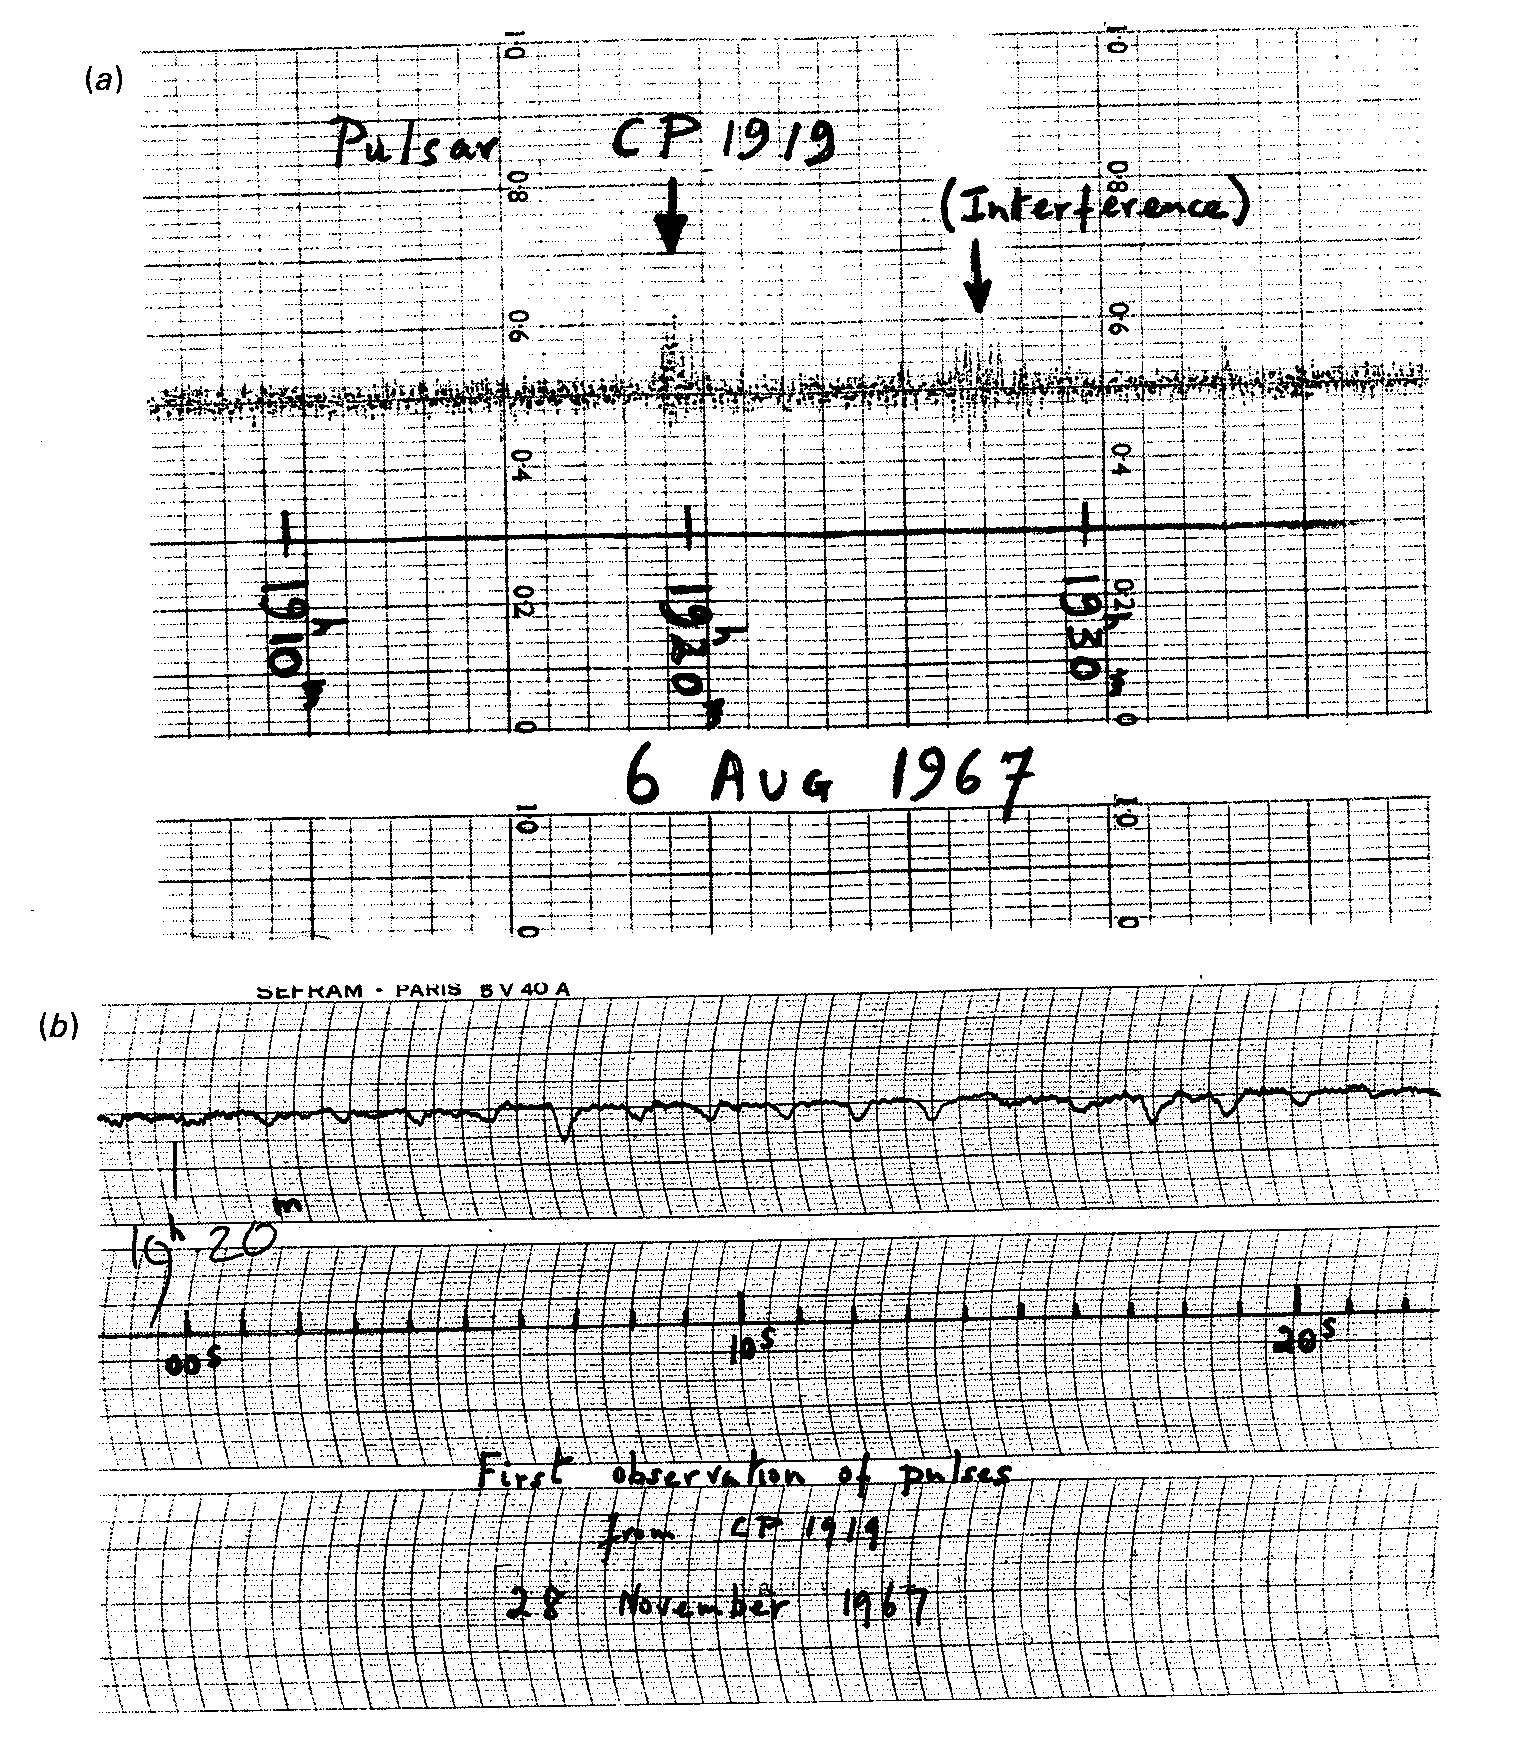
\includegraphics[width=1.0\textwidth]{psr.JPG}
\caption[First detection of pulsar]{Discovery observations of the first pulsar. (a) The first recording of PSR 1919+21; the signal resembled the radio interference also seen on this chart. (b) Fast chart recording showing individual pulses as downward deflections of the trace. From \citet{hewish1964detection}}
\label{fig:psr}
\end{figure}

\begin{figure}[H] 
\centering    
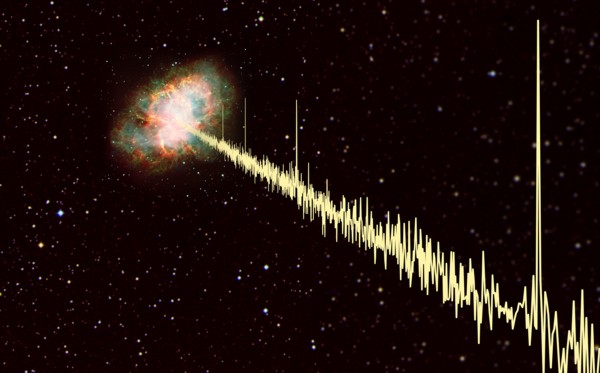
\includegraphics[width=1.0\textwidth]{crab_nebula_pulsar_lo.jpg}
\caption[Crub Pulsar]{The Crab Pulsar and the Crab Nebula are one impressive pair, especially in this unique image made by a duo of NRAO radio telescopes. The Nebula was formed when the original star exploded: this 'supernova' explosion was so bright that in 1054 A.D it was visible in the daytime for several weeks. In the centuries that followed the remnant kept expanding. Then, in 1968, another product of the supernova was found, an object that turned out to be the engine powering the bright remnant: the Crab Pulsar. As the outer layers of the original star were ejected in the supernova, the entire core must have collapsed to form a pulsing neutron star or 'pulsar', one of the densest objects we know of in the entire galaxy.
The image courtesy of NRAO/AUI and Joeri van Leeuwen (UC Berkeley)/ESO/ AURA (\url{http://images.nrao.edu/592}).}
\label{fig:crab}
\end{figure}


\section{Pulsar and Neutron stars properties}
%Add introduction

\subsection{Basic properties}
% Add contents here
\textbf{mass}: The properties of the neutron stars can be deduced by using the equation of stat (EoS),(e.g \citet{oppenheimer1939massive}). Based on EoS model, the maximum mass of the neutron star predicted to be about 2 $M_\odot{}[\footnote{
The minimum and maximum values of the neutron star's masses are vary in the literatures, e.g \citet{lyne2012pulsar} which shows the possible maximum value of the neutron star mass is 3 $M_\odot{}$}]$ (see \citet{lattimer2001neutron}; \citet{lorimer2005handbook}).\\
\textbf{radius and density}: With regard to the neutron star diameters, the mass of many binary systems measured with high accuracy to be $ \approx $ 1.35 $M_\odot{}$. and therefore, the range of EoS for such mass support an equivalent radius in the ranges of 10.5 and 11.2 km. With a similar conditions, the density of the neutron star is $\rho = 6.7 \times 10^{14}$ g $cm^{-3}$ ($>$ density of the nuclear matter $\rho_s = 2.7 \times 10^{14} cm^{-3} $).\\
Consequently, the upper limit of the radius of the neutron star can be deduced by taking into account the stability of the neutron star due to the centrifugal force. For neutron star with mass M and radius R, rotating with angular velocity $\Omega$, for a period $P = 2 \pi/\Omega$ the radius can be given in the form:\\

\begin{equation}
\label{radius}
R = 1.5 \times 10^{3} \left( \frac{M}{M_\odot{}} \right)^{1/3} P^{2/3}km.
\end{equation}

For the fastest known pulsar, PSR J1748-2446ad with the period $P = 1.40$ ms ($\sim 716$ Hz or rotation per second)( 
\citet{hessels2006radio}); consider the mass $m = 1.35 M\odot{}$, this gives a radius of upper limit $R = 21.5$km. \citet{lyne2012pulsar}\\

\textbf{spin-down luminosity}: The lost of rotational kinetic energy is considered to be the reason of the observed spin down that seen on the received pulses, which increases the period of the pulsar as $\dot{P} = \frac{dp}{dt}$. The lost of energy can be given by

\begin{equation}
\label{spin}
\dot E \equiv- \frac{dE_{rot}}{dt} = -I\Omega\dot{\Omega}.
\end{equation}

where $\Omega = 2\pi/P$ is the rotational angular frequency and $I$ is the moment of inertia of the neutron star ($I = 10^{45}$ g $cm^2$), this equation shows the total emitted power from the neutron star.\\

\textbf{spin down and characteristic ages}: The spin down model can be further expressed in terms of rotational frequency ($\nu = 1/P$) by

\begin{equation}
\label{spin down}
\dot \nu = -K \nu^n.
\end{equation}
where K is constant and n is the so-called "braking index" (shows the spin-down behavior of the star and for simplest case, n $\sim 3$).\\
Rewriting equation (\ref{spin down}) in terms of pulse period, $\frac{dp}{dt} \dot{P} = K P^{2-n}$, then integrate and assuming K and n $\neq 1$. therefore, the age of the pulsar can be approximated as

\begin{equation}
\label{age}
T=\frac{P}{(n-1) \dot{P}} \left[1- \left(\frac{P_0}{P} \right)^{n-1}  \right]
\end{equation}
where $P_0 $ represents the spin period at the birth of the star. We can simplify equation (\ref{age}) by assuming $P_{0} << P$ and the spin-down is caused by the  magnetic dipole radiation, n=3 

\begin{equation}
\tau = \frac{P}{2\dot{P}}
\end{equation}

\textbf{Magnetic field}\\
The magnetic moment can be related to the magnetic field strength as $B \approx \frac{m}{r^3}$. then, assuming the neutron star with radius $R=10$ km and the moment of inertia $I = 19^{45} $ g $cm^2$; therefore, we can determine the magnetic field of the pulsar in terms of their period and period derivatives as the following,

\begin{equation}
B = 3.2 \times 10^{19}G \sqrt[]{P \dot{P} }.
\end{equation}
 

\subsection{Rotating dipole model}
The pulsar is a rotating Neutron star with a very strong magnetic field which emits radiation in the different electromagnetic spectrum. Although the emission mechanism of the pulsars has not fully understood yet, many models have been proposed to explain their mechanism. The first model was made by \citet{goldreich1969pulsar}. In this model, the neutron star assumed to have a dense magnetosphere; however, the particles within the region will be electrostatically accelerated by the strong magnetic field lines. The particles then gain energy, due to the acceleration, to escape through the open field lines. see Figure (\ref{fig:dipole model1})

\begin{figure}[H] 
\centering    
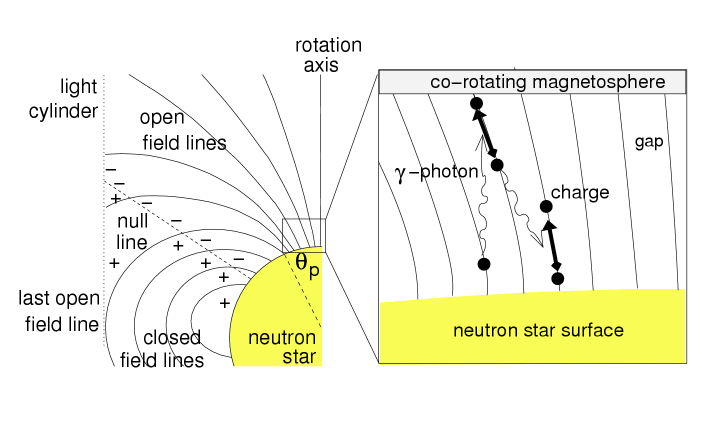
\includegraphics[width=0.8\textwidth]{JLmodel.png}
\caption[The Goldreich-Julian Model
Goldreich]{Illustrates how the process of the emission mechanis
m from the polar gab with the electon-positron cascade.
Figure from Hand book pulsar astronomy by \citet{lorimer2005handbook} }
\label{fig:dipole model1}
\end{figure}

Following the first model (\citet{goldreich1969pulsar}), the second attempt was carried by \citet{sturrock1971model} when he proposed a new mechanism of the "polar caps" (the area where the open field lines reached the light cylinder and connect with the surface of the star). however, each polar cape has electrons and protons polar zone. The electrons then accelerated along the open magnetic-field lines which leads to produce a $\gamma$ ray emission due to the curvature radiation. If the pulsar with a short period, $> 1$ second, the pairs of the electron-positron will be constructed and accelerated, for the second time, to produce more emission in the form of pair cascade. Furthermore, \citet{ruderman1975theory} also proposed a new model related to the previous one (e.g \citet{sturrock1971model}). The new model is the so-called the "polar gap model" which suggested that the open field lines are extended to high altitude from the stellar surface by the polar magnetosphere gap. This will create a difference between the top and the base of the gap, as the result, the gap "spark" by generating electron-positron pairs which allow the emitted emission to be observed. see Figure (\ref{fig:dipole model})

\begin{figure}[H] 
\centering    
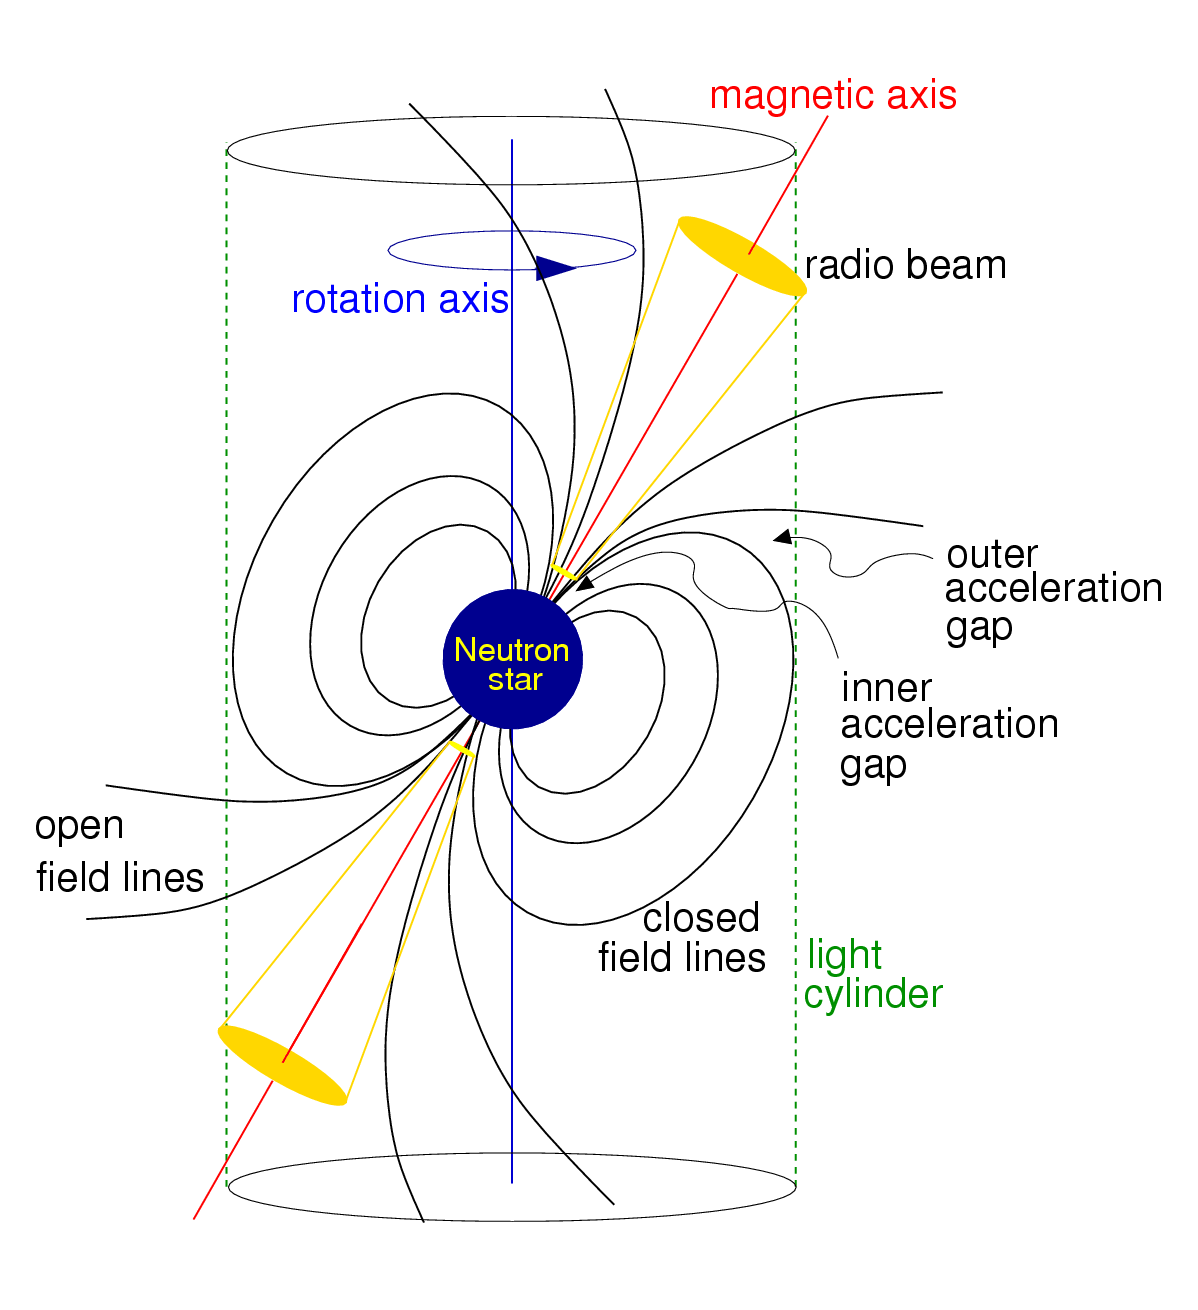
\includegraphics[width=0.8\textwidth]{PSRs_pulsar_sketch.png}
\caption[magnetosphere model]{Shows the rotating dipole of the pulsar emission.
Figure from Hand book pulsar astronomy by \citet{lorimer2005handbook} }
\label{fig:dipole model}
\end{figure}


\subsection{Galactic distribution}
\label{GD}
The standard model of neutron stars formation proposed that the neutron stars are the result of supernova explosions of massive stars (\citet{lyne1994high}). More than 2600 pulsars are now known (\footnote{This is ATNF Pulsar Catalogue, version:1.57 \url{http://www.atnf.csiro.au/research/pulsar/psrcat/}}). Figure (\ref{fig:GD}) indicates that most of the pulsars are located near the center of the galactic plane which supports the standard model of the birth of neutron stars. In 1970 \citet{gunn1970nature} formulated a statistical method to study the magnetic-dipole model of pulsar's observations which leads to the first suggestion about the high-velocity of the pulsars using the existence of both, the proper motion in the Crab Nebula and the O-B stars as anomalously massive stars category as evidence to support this idea. By analyzing the distribution of pulsars perpendicular to the galactic plane, the authors found that the pulsars are likely born with a velocity of $100^{-1}s$ which agree with the previous dynamic hypothesis. This implies a "kick" during the birth depending on the edge of the object and similarly, it explains why the young pulsars are close to plan and the old luminous pulsars with the very long period appear far away from the galactic plane with an isotropic distribution. (see the open circle in Figure (\ref{fig:GD}) ), this known as Millisecond Pulsars. Subsection (\Cref{MSP}). 

\begin{figure}[ht!] 
\centering    
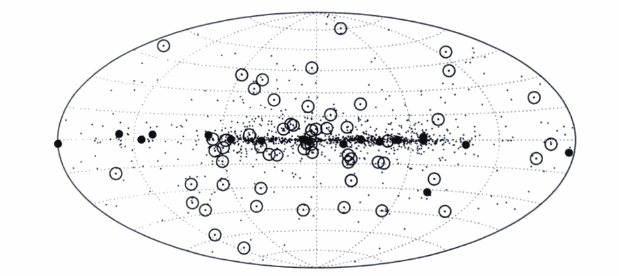
\includegraphics[width=1.0\textwidth]{GD.png}
\caption[Galactic Distribution of pulsars]{Shows the Hammer-Aitoff projection of the sky in Galactic coordinates. The filled circles show the Pulsar-supernova and the open circles show the millisecond pulsars. Image from Handbook of Pulsar Astronomy
book }
\label{fig:GD}
\end{figure}

\section{Pulsar categories and their evolution}
%NOTE to add the ref for different section 
\subsection{ \texorpdfstring{$P-\dot{P}$}{} Diagram}
The observed emission from pulsars, which is a result of the rotational kinetic energy of the neutron star, enables us to measure the pulsar's spin period, P, and the correspond spin-down rate, $\dot{P}$, of the pulsar with very high precisions measurements. Using a smiler idea of Hertzsprung- Russell diagram to study the evolution of the stars by plotting the luminosities versus the stellar classifications, the $P-\dot{P}$ diagram gives us an excellent overview of the spin evolution and other properties of the neutron stars by plotting the period and it's derivative (P and $\dot{P}$ respectively). Figure (\ref{fig:pp}) shows different types of pulsars, In the center we see the normal pulsar population (\cref{Normal Pulsars}) with the black dot, they are young and slow. Upper right we see the highly magnetized neutron stars called Magnetars with the green triangle. Button left show the binary system of pulsar which the origin of Millisecond Pulsars. We see also different types of pulsars associated with supernova remnants present by blue squares. Finally, we can note the yellow squares which show the Rotating Radio Transients.

\begin{figure}[H] 
\centering    
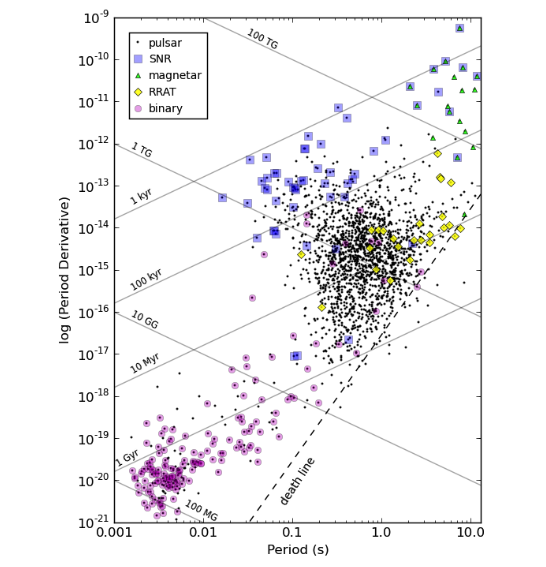
\includegraphics[width=1.0\textwidth]{sallycooper.png}
\caption[P--$\dot{P}$ Diagram]{: P--$\dot{P}$ diagram for known pulsar until 2016, the black dot in the middle right present the Normal pulsars "island", blue squares shows pulsars associated with supernova remnant (SNR), the purple circles in lower left shows the millisecond pulsars, the yellow poxes in the center to the right show the Rotating Radio Transients (RRATs) where the green triangle in the top right show the highly magnetize type of pulsars called Magnetars. Image made by \url{Sally_ Cooper}}
\label{fig:pp}
\end{figure}


\subsection{Normal pulsars}
\label{Normal Pulsars}
From the diagram in Figure (\ref{fig:pp}) it's clear that normal pulsars have surface magnetic field strength an order of $~10^{11}$ to $~10^{13}$ G, spin period of 0.1 to 1.0 second and period derivatives in order of $~10^{-16}$ to $~10^{-14}$ s $s^{-1}$. The normal pulsars have short spin period when they form (at the upper left-hand in Figure (\ref{fig:pp})), then followed by spin down and as a result, they move  toward the center (pulsar island) to have a characteristic ages $~10^{5}$ to $~10^{8}$ Years in their evolutionary tracks until finally, they become very faint to be detected after ~$10^{8}$ yr. More information about the characteristic of the normal pulsar can be found in (\url{https://arxiv.org/abs/astro-ph/0208557v1}).  

\subsection{Millisecond pulsars}
\label{MSP}
The second class of the pulsar populations with very short period and high spin frequency rate is so-called Millisecond Pulsars. As we look at Figure (\ref{fig:pp}), we can clearly spot the unique location of the millisecond pulsars population in the left button of P--$\dot{P}$ diagram with the magnetic field $10^{8}$ G and characteristic ages $10^{7}$  yr. One of the mean properties of millisecond pulsars is that they have orbiting companions observed at around 80\% of the total number of millisecond pulsars compare to 1\% for the normal pulsars. These orbiting companions could be one of the following, mean sequence stars, white dwarfs or neutron stars.\\
Following a similar evolutionary track of the normal pulsars discussed in (\cref{GD}), when the pulsar in the binary system last over $~10^{7}$ yr, it becomes faint (the energy of the star decreases and thus insufficient radio emission will be released), and undergo spin down which will become very slow with spin period in order of several seconds only. The model of the binary system formations has proposed to describe the formation of millisecond pulsar (\citet{alpar1982new}).\\
The formation and evolution model for different binaries has shown in figure (\ref{fig:mspf}), as the pulsar in the binary system spin down, some binary systems remain bounded with their companions. The massive companion then expands and evolve to become a giant star, as a result, the distance between the pulsar and its companion will decrease which enables the companion to fill it's Roche Lobe and accrete the matter (and subsequently transfers the orbital momentum) into the old neutron star to create an accretion disk. the pulsar start spinning up again for short periods, this is also called "recycled pulsar". in this stage the X-rays emission will be released and the system is called X-ray binary.\\
Depending on the mass of the companion, two classes can be identified, high-mass X-ray binaries ($HMXB_{s}$) and low-mass X-ray binaries ($LMXB_{s}$). In the case of the $HMXB_{s}$ shown in the sketch (\ref{fig:mspf}), the massive companion will continue evolving to explode as a supernova, forming a second neutron star. this system is called Double Neutron Stars. The first discovery of such system has curried by \citet{taylor1982new}. PSR J0737-3039 system (\citet{burgay2003increased}) is the first double neutron system to be observed as binary pulsars. with 22 ms period and an orbital period of order 2.4 hours, this makes it one of the best system to be used in testing the theory of general relativity and other theories of gravity. $HMXB_{s}$ can also form neutron star-black hole binary or even a black hole binary.\\
For the $LMXB_{s}$ case, the system evolves to be millisecond pulsar-white dwarf binary system.
For full review see (\citet{Lorimer2001})  
(\citet{backer1982millisecond})

\begin{figure}[H] 
\centering    
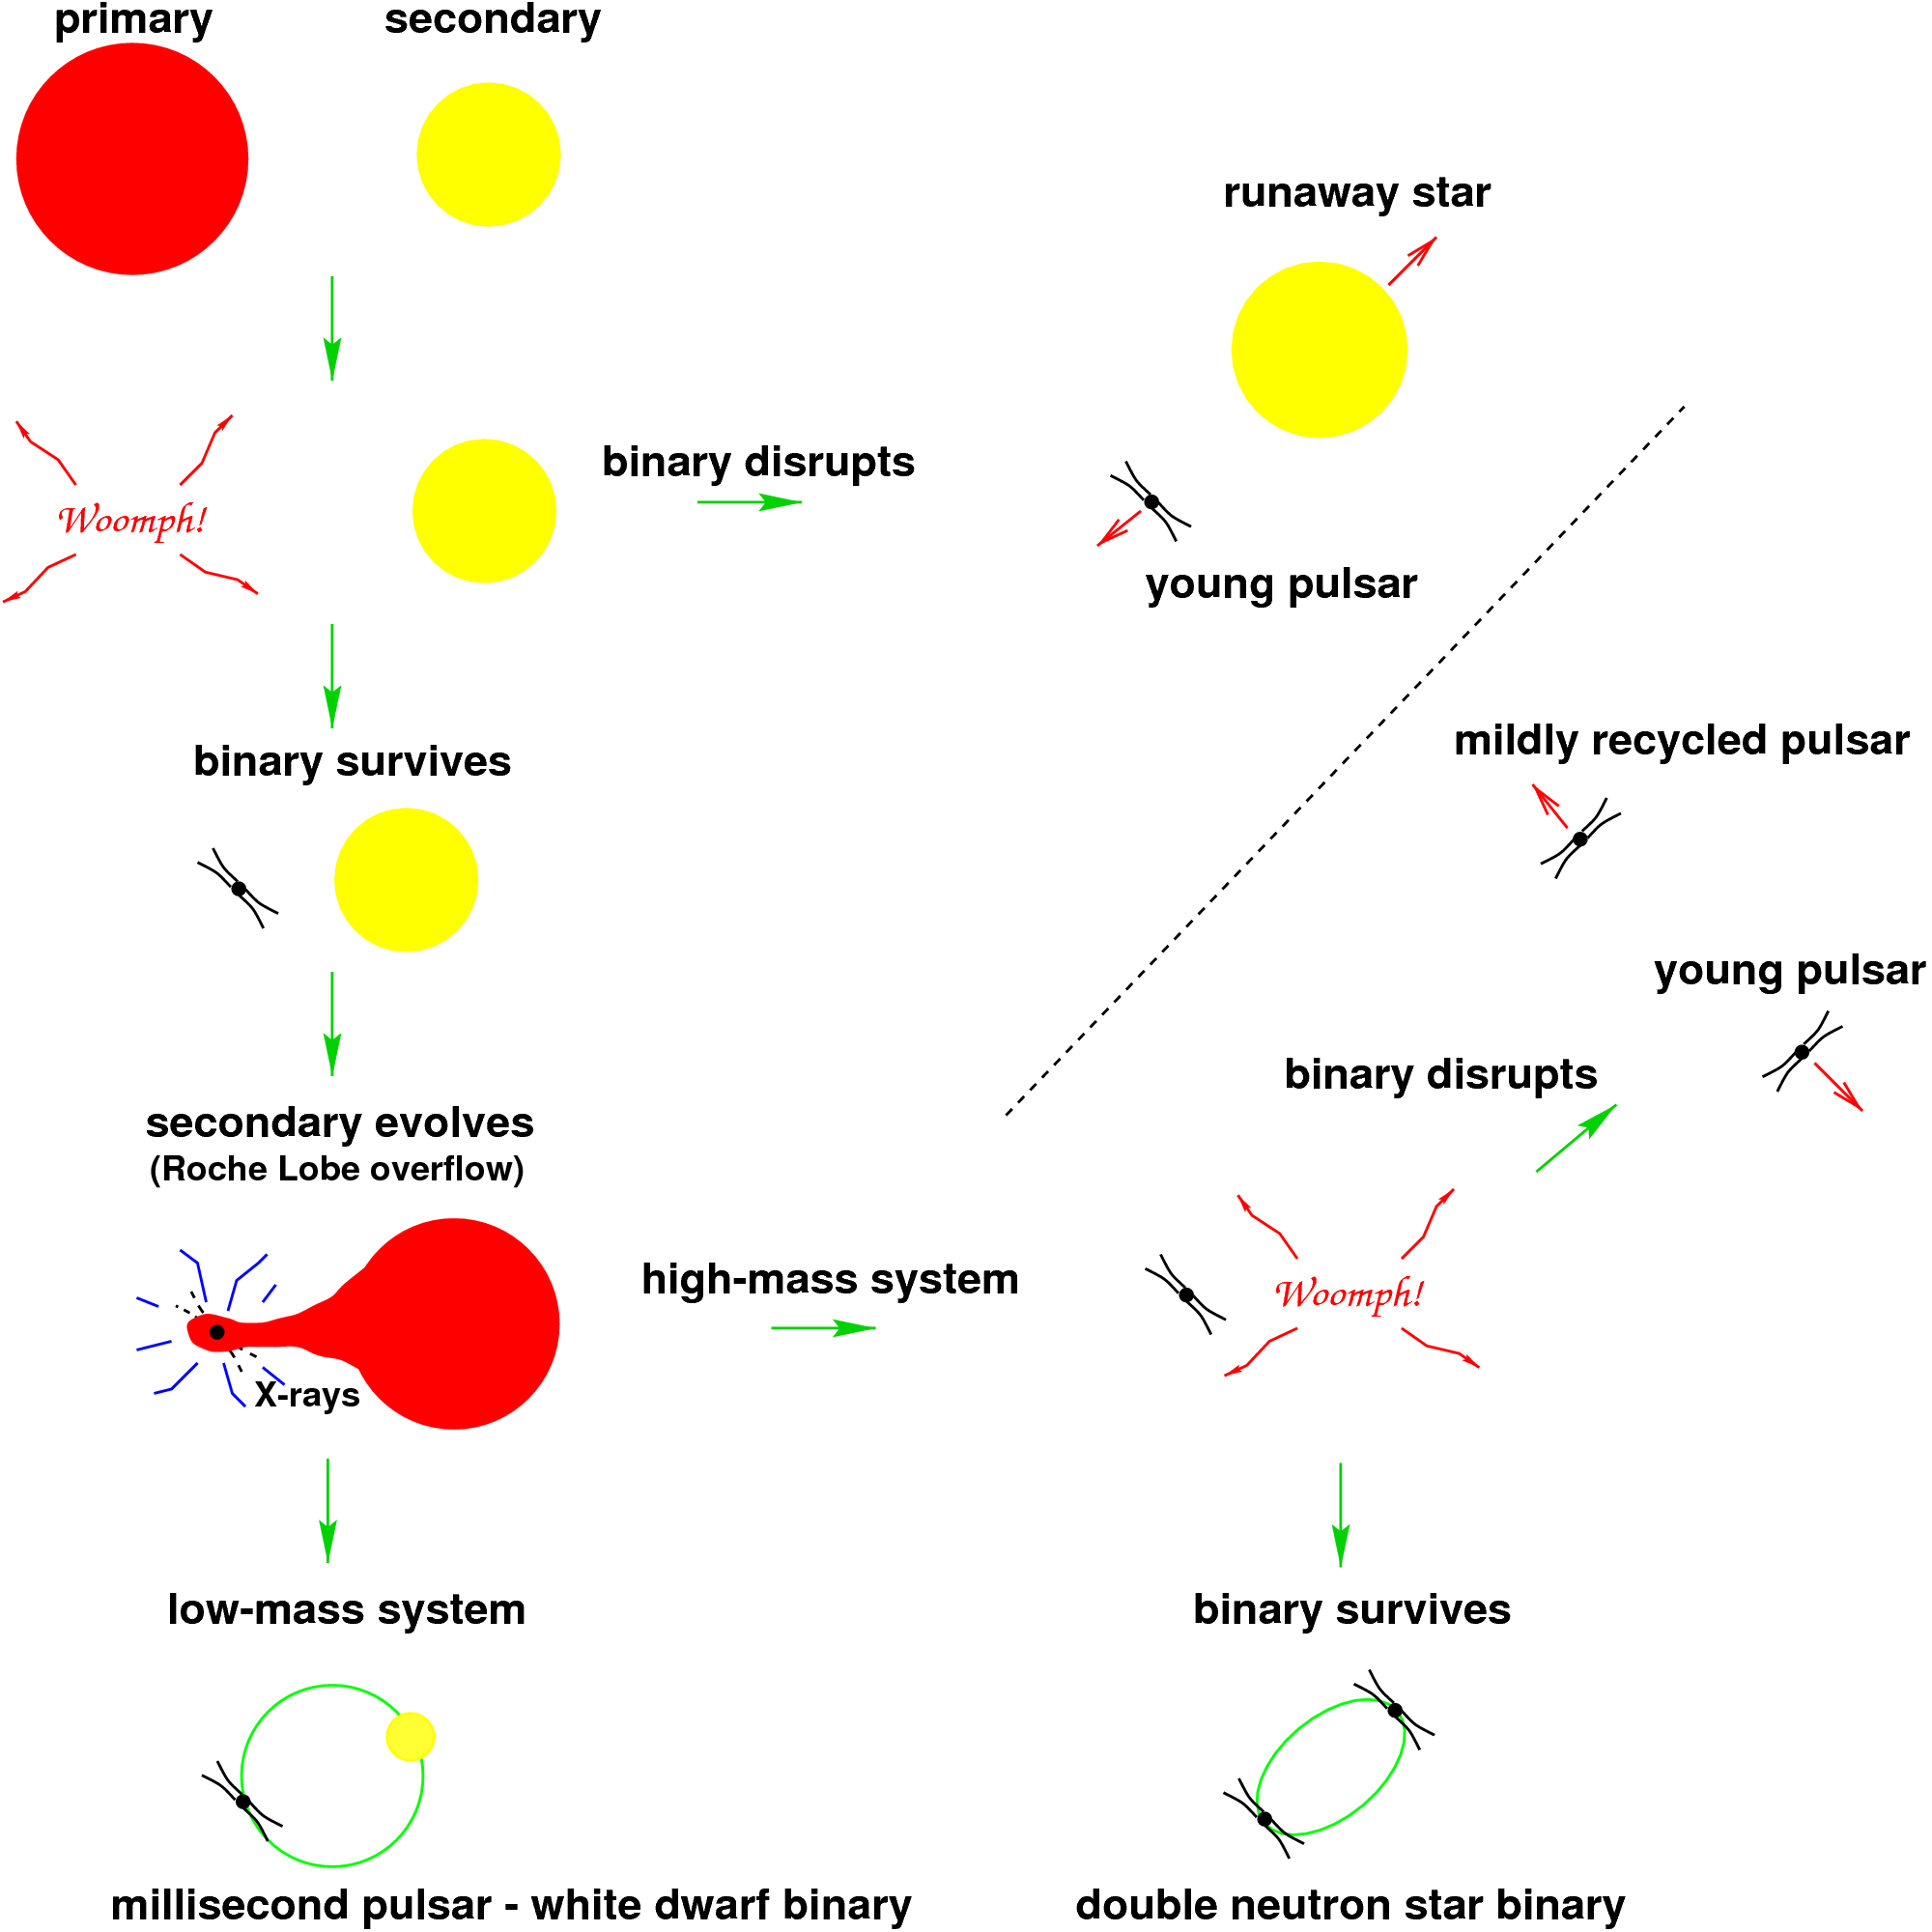
\includegraphics[width=1.0\textwidth]{MSformation.png}
\caption[Formation model of the Binary system]{Shows the formation and evolution of different types of binary systems, The image from \citep{Lorimer2001}  
}
\label{fig:mspf}
\end{figure}


\subsection{Magnetars}
Another type of pulsar with an ultra-magnetic field is the "Magnetars". They located in the upper right-hand of Figure (\ref{fig:pp}) shown by the green triangle, with magnetic field strengths of order $B \sim 10^{15}$ Gauss, which makes them one of the strongest cosmic magnetic field object in the universe. As suggested by \citet{thompson1993neutron}, the decay of magnetic field is considered to be the main source of magnetar energy, the magnetar model \footnote{\citet{duncan1992formation} for more details in different possibilities of the model}. They concluded: " Magnetic fields can deposit an enormous amount of energy outside a young neutron, and can catalyze the conversion of energy from neutrinos to electron pairs".\\
Depending on their observed emissions, two types of magnetars have been classified: Soft gamma repeaters (SGRs) which identified as high-energy transient sources. The second class is what called Anomalous X-ray pulsars (AXPs) which show continuing pulsation with rapidly spinning down in X-ray ranges, as well as some, have been observed as SGR-like bursts source. These two classes have spin period between 5 to 12 seconds and very short characteristic ages in order $ P / \dot{P} \sim 10^{3} - 10^{5}$ yr. (For full review see the book \citet{lewin2006compact}. Magnetars also have been observed as radio pulsar in the system \textbf{XTE J1810-197} which emits bright, narrow radio pulses with very high linear polarization (\citet{camilo2006transient}.%(\citet{israel2004accurate})


\subsection{Rotating Radio Transient (RRATs)}
Anew type of pulsars populations can be identified as the Rotating Radio Transients (RRATs), the yellow pox in the center to the right of Figure (\ref{fig:pp}). The discovery of the RRATs has been carried by \cite{mclaughlin2006transient} when eleven sources were identified as single pulses of radio emission using data from Parkes Multi-beam Pulsar Survey. The measure duration of these pulses range between 2 to 30 ms with flux density peak ranging from 0.1 to 3.6 Jy, while the average time interval between the burst found to be in order of 3 minutes to 3 hours, as well as the dispersion measure (DM) value which shows a constant value for all the eleven sources.



For full review see \citet{2010PhDT.......460K}







%********************************** %Second Section  *************************************

\section{Interstellar medium (ISM)} %Section - 1.2
\label{ISM}

%Add some more contents

The interstellar medium (ISM) is the environment between the star systems in a galaxy that contains ordinary matter, relativistic charged particles (cosmic rays) and magnetic field. The standard model consists of three components which are in pressure equilibrium. Two of these components were suggested by \citet{field1969cosmic} which are based on heating by low-energy cosmic rays, the cold dense phase $T < 300 K$ which consists of neutral and molecular hydrogen clouds and warm intercloud phase $T = 10^{4} K$ consisting ionized gas. The third phase is the hot ionize gas with temperature  $T = 10^{6} K$  which has been added by \citet{mckee1977theory}. their study showed that the hot ionized gas is a result of the supernova explosions which create a shock-waves that evaporate the cool clouds to hot medium.\\
As the radio emission from pulsars propagates through the ionized interstellar medium (\textbf{ISM}), it interacts with the free electrons leading to observable propagation effects. There are three main effects that affect the signals (pulses) from the pulsar traveling through the ISM: scintillation, scattering, and dispersion. To create a high precision timing, one needs to correct for these effects (e.g. \citet{armstrong1995electron})




\subsection{Dispersion}
\label{Dispersion}
As we mention in \cref{ISM}, the frequency dispersion is one of important characteristic of the radio signals from pulsars, when they propagate through the ionized interstellar medium. The refractive index of the gas in the ionization state can be obtained from the plasma frequency $\nu_{p}$ as,

\begin{equation}
\label{revractive index}
n = \left(1- \frac{\nu^{2}}{v^2} \right)^2
\end{equation}

and thus,the plasma frequency is \footnote{The electron density in ISM environment is given in $cm^{-3}$ which also can represent in kHz. As the approximate value of $n_e=0.03 cm^{-3}$ gives a plasma frequency of 1.5 kHz, then we can approximate the refractivity (n-1) to be $-2.4  \times10^{-10}$ for a 100 MHz. see the book for full text \cite{lyne2012pulsar} }  

\begin{equation}
\label{revractive index1}
\nu_p^2 = \frac{n_e e^{2}}{\pi m}
\end{equation}

where n is the refractive index of the ionized gas and $\nu$ is the frequency of the wave. e and m are the electronic charge and mass respectively. As the group velocity of the traveling pulses is $\nu_g = cn$, where c is the speed of light in the vacuum, thus for the given electron densities 

\begin{equation}
\label{group velocity}
\nu_g^2 = c \left(1 - \frac{n_e e^{2}}{2\pi m v^2} \right)
\end{equation}

The travel time T through the distance L, therefore, will be in the form 

\begin{equation}
\label{Travel Time}
T = \int_0^L \frac{dl}{v_g} = \frac{L}{c} + \frac{e^2 \int_0^L n_e dl}{2 \pi mcv^2}  = \frac{L}{c} + 1.345 \times 10^{-3} v^{-2} \int_0^L n_e dl  
\end{equation}

This equation shows the travel time of the free space (the first term) with an additional term which represents the dispersive delay t. the 
extra term is the what called the dispersion measure (DM)\footnote{The unit of the DM is a combination of the distance unit, parsecs = 3 $\times10^{18}$ and  the unit of the density, $cm^{-3}$ } given as

\begin{equation}
\label{Dispersion measure}
DM =  \int_0^L n_e dl
\end{equation}

Which measures the electron density between the pulsar and the telescope, with unit $ cm^{-3}$ pc.

From equation \ref{Travel Time} and \ref{Dispersion measure}, the delay due to dispersion can be written in the form 

\begin{equation}
\label{Dispersive Delay}
t =  \mathcal{D} \times \frac{DM}{\nu^2}
\end{equation}

Where $\mathcal{D}$ is the dispersion constant which given as 

\begin{equation}
\label{Dispersion Constant}
\mathcal{D}  = \frac{e^2}{4 \pi mc} = 4.1488 \times 10^{3} MHz^{2} pc^{-1
}cm^3
\end{equation}

If we have tow different frequencies ($\nu_{low}$ and $\nu_{high}$), then equation \ref{Dispersive Delay} can be written in another useful form as

\begin{equation}
\label{Dispersive Delay of two freq}
\Delta t =  \mathcal{D}.DM \times \left(\frac{1}{\nu^2_{low} } - \frac{1}{\nu^2_{high} } \right)
\end{equation}

The effect of this delay can be seen in the observations when the pulses with higher frequencies arrive earlier than that in low frequencies as shown in Figure (\ref{fig:DM effect}). The time differences of the received signal with bandwidth B (in MHz) can be calculated (in seconds) as

\begin{equation}
\label{Disp}
\Delta t =  8.3 \times 10^3 DM \nu^2 B 
\end{equation}


\begin{figure}[htbp!] 
\centering    
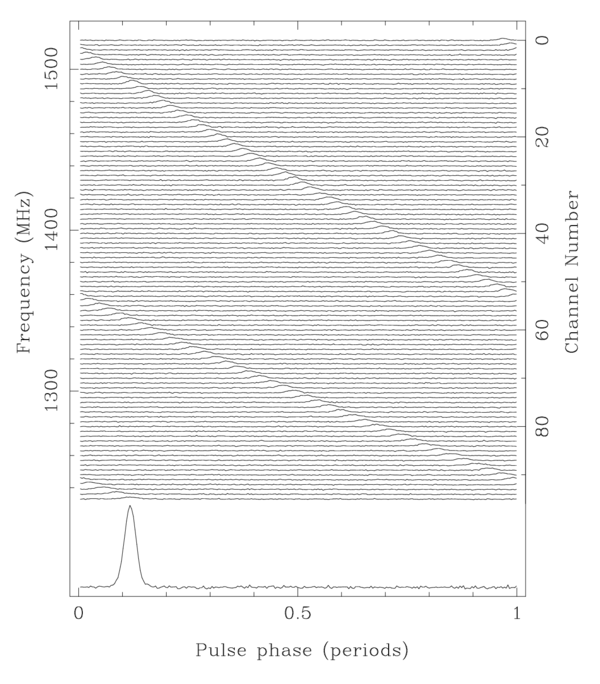
\includegraphics[width=0.8\textwidth]{pulsar_dm.png}
\caption[The frequency dispersion]{Shows the effect of the frequency dispersion which the pulses at high frequencies  arrive earlier for PSR B1641-45. The image from \citet{lyne2012pulsar}.  
}
\label{fig:DM effect}
\end{figure}

%The dispersion can be used to measure how far the pulsars are located from the earth. As the value of DM can be determined by measuring the distribution of the free electrons, \citet{2002astro.ph..7156C} have described a new model "NE2001" to approximate the distance of the pulsars.\\


\subsection{De-dispersion}
%Add section for the dm variation and another for structure function 
We have discussed in section \cref{Dispersion} the effects of the dispersion on the radio pulses source which causes the pulses at high frequencies arrive earlier than that at low frequencies. When the dispersive delay becomes larger than the period of the pulsars, the detection of a new pulsar will become more difficult. Therefore, we need to solve this effects. The method used to solve this effect is called the \textit{de-dispersion} and can be implemented by two way

\subsubsection*{Incoherent de-dispersion}
This method uses the technique of separating the received bandwidth into multiple sub-bands and then apply a suitable delay for each channel. This delay will adjust the channels to be aligned along the range of frequency and solve for the delay Figure (\ref{fig:de-DM}) (e.g \citet{large1971search}) 

\begin{figure}[htbp!] 
\centering    
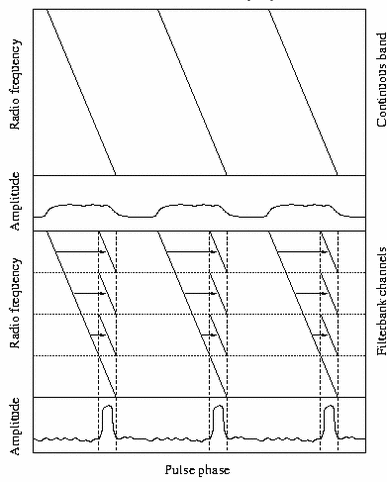
\includegraphics[width=0.8\textwidth]{de_dm.png}
\caption[The de-dispersion]{Shows the broadened profile of the received pulses due to dispersion (top panel). The process of solving the dispersion delay by dividing sub-band into multiple channels and apply the suitable delay for each channel (lower panel).
Figer from Hand book pulsar astronomy by \citet{lorimer2005handbook} }
\label{fig:de-DM}
\end{figure}



\subsubsection*{Coherent de-dispersion}
This technique applies the processing of the full bandwidth signal before the detection, therefore, removing the effect of the interstellar dispersion with higher precession than incoherence techniques (e.g   
\citet{rickett1975radio}). This can be achieved by applying a phase delay, correspond to specific frequency, to the received signal in the filter. The filter then digitizes the signal before the detection by applying the Fourier transform techniques to a sequence of samples. Then, the phase in each discrete components of the spectrum can be delayed by appropriate values depending on the amount of the frequency. Finally, the reverse Fourier transform is used to return the signal the signal without the dispersion delay \citet{lyne2012pulsar}.      


\subsection{Scattering}
We outlined in section \cref{Dispersion} the dispersion effects of the radio pulses from pulsars when they pass through the ionized ISM, however, the inhomogeneities of the electron density along the line of sight causes scattering of the pulses. The mean effect of the inhomogeneities on the observed pulses causes broadening the pulses in time, therefore, a simple model of a thin screen was proposed by \citet{williamson1972pulse}. In this model, the scattered electrons along the line of sight from the pulsars to an observer leads to frequency dependence effect such as the pulse broadening Figure (\ref{fig:scut_model}).\\
As the wave propagate through an inhomogeneity, its phases change due to the refractive index and thus, by consider a screen with scale a in the midway between the pulsar and the observer, we can manifest this phase change $\Delta\theta$ by approximate the angle $\theta_0$ at the screen as

\begin{equation}
\label{angle}
\theta_{0} \approx \frac{\Delta\theta / k}{a} \approx \frac{e^2}{\pi m_e} \frac{\Delta n_e}{\sqrt{a}} \frac{\sqrt{D}}{f^2}
\end{equation}

where $k = (2\pi/c) \mu f$ and D is the distance to the pulsar\\
Similarly, an angular radius $\theta_d$ of the diffuse scatter disk around the source can be seen by an observer as

\begin{equation}
\label{anglular}
\theta_{d} = \frac{\theta_0}{2} \approx \frac{e^2}{2\pi m_e} \frac{\Delta n_e}{\sqrt{a}} \frac{\sqrt{D}}{f^2}
\end{equation}

the angular intensity distribution also observed to follow the gaussian probability distribution as 

\begin{equation}
\label{intinsity}
I(\theta)d\theta \approx \exp(-\theta^2/\theta^2_D) 2 \pi \theta d\theta
\end{equation}

The received scattered-waves therefore will travel an additional distance, due to the small change in the direction (see Figure \ref{fig:scut_model}), and thus the path length will also increase which eventually leads to a geometrical time delay $\Delta t(\theta)$ as

\begin{equation}
\label{g delay}
\Delta t(\theta) = \frac{\theta^2 D}{c}
\end{equation}

This effect can be used to obtain the observed intensity, I, as a function of time

\begin{equation}
\label{obs-intinsity}
I(t) \approx \exp(-c \Delta t/(\theta^2_d D)) \equiv e^{-\Delta t/\tau_s}
\end{equation}

Where

\begin{equation}
\label{tau}
\tau_s = \frac{\theta^2_d D}{c} = \frac{e^4}{4 \pi^2 m^2_e} \frac{\Delta n^2_e}{a} d^2 f^{-4}
\end{equation}
This what shows the observed tail with the exponential shape that appear on the received pulse signal. 


\begin{figure}[H] 
\centering    
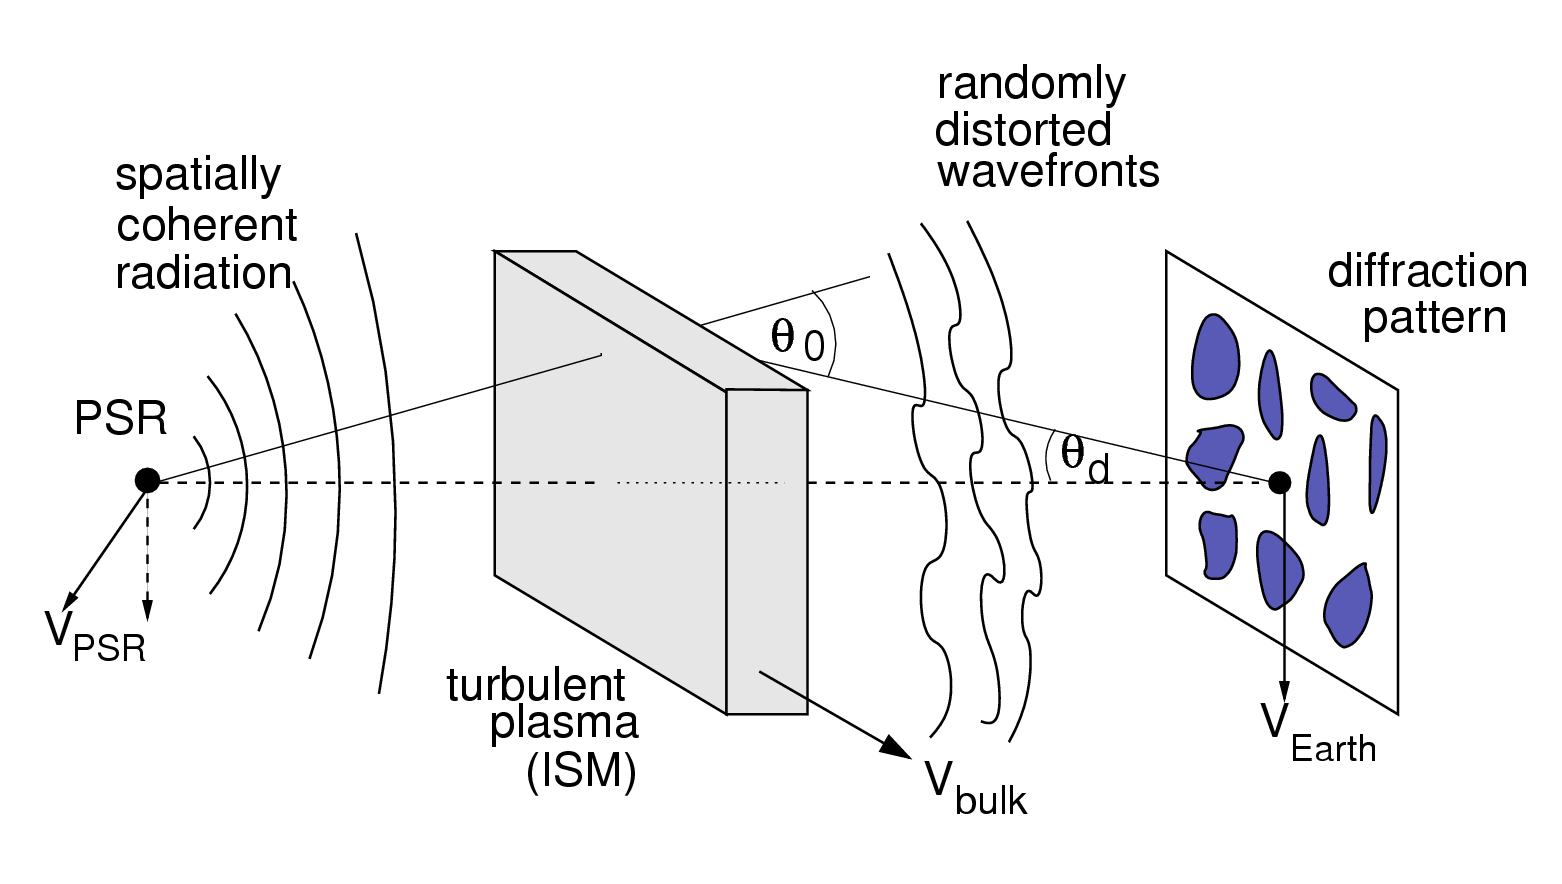
\includegraphics[width=0.85\textwidth]{PSRs_thin_screen.png}
\caption[The de-dispersion]{Shows the broadened pulses due to screen scattering model.
Figure from Hand book pulsar astronomy by \citet{lorimer2005handbook} }
\label{fig:scut_model}
\end{figure}


\subsection{Scintillation}
Beside the dispersion and scattering of the ISM, an additional effect called "interstellar Scintillation" also can be observed. The scintillation is defined as a short-term intensity variation appear on the pulsar observations. This caused by the random electron density between the pulsar and the observer.\\
Using a similar model of the scattering, the thin screen model can be used for analysis
of the pulsars scintillation. Figure (\ref{fig:sscint_model}) shows that the scattered radiation from the pulsar to an observer presented in a thin screen leads to random irregularities in the refractive index which causes phase variations of the wavefront. This phase differences then will be received along the line of sight by the observer as a scintillation pattern.\\
The scintillation bandwidth $B_{s}$ can be given by the simple formula

\begin{equation}
\label{dm scintillation}
B_{s} \approx \frac{8 \pi^2 a c}{D^2 (\Delta n_e)^2 \lambda^4}
\end{equation}

Where D is the distance between the pulsar and the observer, a is the length of the scattered ray path, c is the speed of light and $\lambda$ is the wavelength (\citet{lyne2012pulsar}).

\begin{figure}[H] 
\centering    
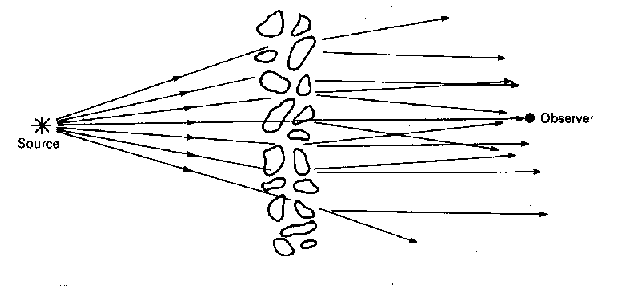
\includegraphics[width=0.85\textwidth]{scintt.png}
\caption[scintilation]{Shows the random irregularities of refractive index as represented by thin-screen model of scintillation}
\label{fig:sscint_model}
\end{figure}


%********************************** % Third Section  *************************************
\section{Pulsar timing}  %Section - 1.3 
\label{section1.3}
%#####Add more about in pulsar timing. why do we do pulsar timing?
Pulsar timing is a technique used to study the spin evolution of the pulsars by measuring the time of arrival (TOAs) of the transmitted pulses from pulsars to the Earth. Study and analyze TOAs allow us to deliver research and knowledge in many areas. first, studying the origins of the pulsars and construct the properties associated with it (e.g period, spin and spin down, age, etc), second, using pulsars as a tool to measure the positions of the source with high accuracy values, third, exploring the propagation of the pulses through the ISM; therefore, many effects of ISM can be studied (e.g dispersions of the pulse, see \ref{Dispersion}).\\
Similarly, apply pulsar timing on the pulsars in a binary system enable to measure their orbits and rotations slowdown and testing the Einstein's theory of Relativity. One of the main applications of pulsar timing also, to detect low-frequency gravitational waves (e.g stochastic background). In this section, we give overview of pulsar timing techniques, TOAs and timing model and its parameters.\\
this section is based on \citet{lorimer2005handbook} and the recent review from \citet{manchester2017pulsar}\\


%Pulsars are rotating neutron stars that emit beams of radiation in the different spectrum (e.g radio, optical, X-ray and $\gamma$-ray). , time of the writing, with periods (Ps) range between 1 ms to 15 s. Different categories of pulsars vary on their parameters. Milliseconds \Cref{MSP}, for instance, have short Ps, 1 ms to 10 ms and very small period derivative or the so-called "slowdown rate", ($\dot{P}$). On the other hand, Normal pulsars \cref{Normal Pulsars} have long Ps, 3 s to 0.3 s. ===========

%########## its repeated
%######### Now there is a pulsar with period of 33.05s. new paper but not published yet

\subsection{Time of arrivals (TOAs)}
The time of arrival (TOA) is defined as "the arrival time of the nearest pulse to the mid-point of the observation" \citet{lorimer2005handbook}. In pulsar timing, the TOAs taken from pulsars observations over long interval enable us to create a timing model; which then can be used to determine the parameters of the pulsars, with a good accuracy, and perform the analyses of their evolution.\\
Practically, to measure the arrival times of the pulses, the pulsars data need to be folded at the period of the pulsars. the result of this process is the so-called "average pulse profile" which used to establish the timing.

\subsection{Template matching}
\label{cross-correlation}
The generated average pulse profile is very stable and therefore, the TOAs can be determined with high accuracy. The cross-correlation method is considered the best methods for measuring the timing of arrival of pulsars. In this methods, the observed profile is matched with high signal to noise (S/N) template. these templates are constructed from a set of early observations at a known range of frequency.\\
Suppose the average pulse profile is given by $\mathcal{P}(t)$, $\mathcal{T}(t)$ for the template and noise $\mathcal{N}(t)$ thus

\begin{equation}
\label{cross-cor}
\mathcal{P}(t) =  a + b \mathcal{T}(t - \tau) + \mathcal{N}(t)  
\end{equation}

where a is the arbitrary offset and b is scaling factor and $\tau$ is the phase offset which shows the time-shifted between the template and the profile; then by applying the cross-correlate technique, TOAs can be measured.\\
TOAs can be measured with high precisions; however, many effects, either associated with the pulsars or as systematic effects, can limit the measurements of pulsars TOAs. This introduces an uncertainty in the measurements of TOAs which can be calculated by the following formula

\begin{equation}
\label{toa precision}
\sigma_{TOA} \simeq  \frac{S_{sys}}{\sqrt[]{t_{obs} \Delta f}}  \times \frac{P\delta^{3/2}}{S_{mean}}
\end{equation}

Where $S_{sys}$ is the flux density of the system, $\Delta f$ is the observed bandwidth, P is the pulse period, $\delta = W/P$ is the pulse duty cycle and the mean flux density is given by $S_{mean}$.





\subsection{Pulsar timing-model parameters}
%check the range approx of the values for each parameters
In the pulsar timing, the measured TOAs from the received pulses at the observatory needs to be fitted to a model by using an appropriate method (e.g cross-correlation Section \ref{cross-correlation}). Considering this fitting, there will be variations between the TOAs at the telescope and the time of emission at the pulsar; hence, a timing model is required to correct all the effects which limit our ability to measure the average TOAs with high accuracy.\\
Here we show some of the parameters of the timing model and how they appear in the timing residuals of the observations (Figure \ref{fig:timing model}) . For full review see \citet{edwards2006tempo2}


\begin{figure}[H] 
\centering    
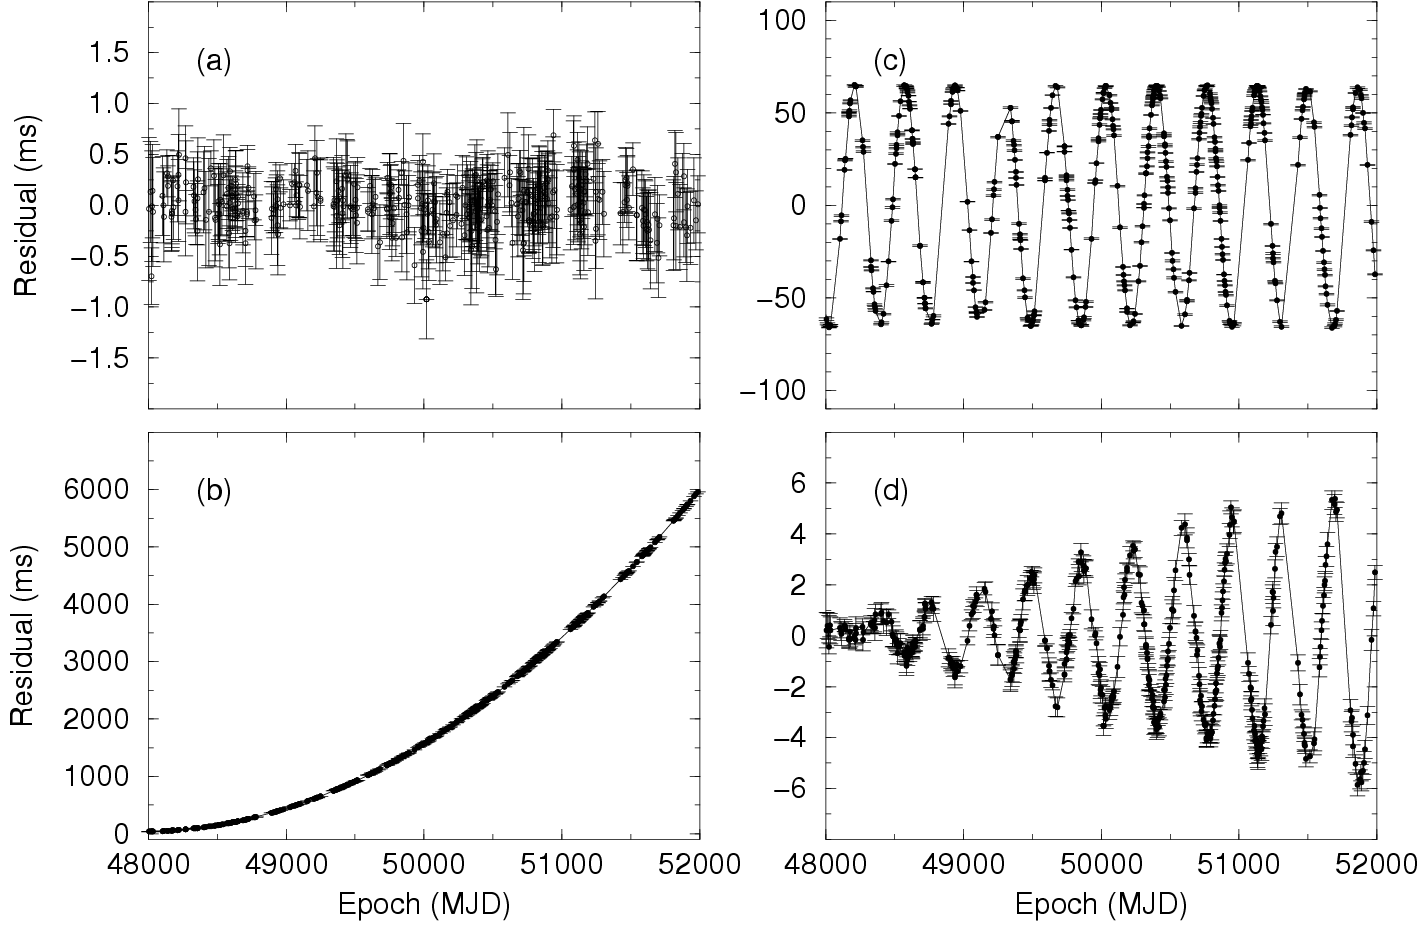
\includegraphics[width=0.85\textwidth]{PSRs_timing_example.png}
\caption[scintilation]{Shows timing-model parameters and their effects on the residual structure. Panel (a) shows an accurate timing model which all the residual centered around 0 ms. Panel (b) The spin down (or frequency derivative) errors which give a quadratic increase shape. Panel (c) The position error which gives a sinusoidal shape due to the variation with the period of the Earth around the sun (1 year). Panel (d) shows inaccurate pulsar's proper motion measurements which result in 1-year sinusoid shape with quadratically-increasing amplitude. \citet{lorimer2005handbook}}
\label{fig:timing model}
\end{figure}


\subsection*{Barycentric corrections}
Observatories on Earth measure the pulse TOAs by an atomic time standard called "Terrestrial Time (TT)"; Measuring the TOAs using the observatory clock is known "topocentric arrival time" which occurs in non-inertial frame, due to rotating Earth orbiting the Sun; therefore, we need to transfer this to an inertial reference frame which represents the center of mass for the solar system. The frame of Solar system barycenter "SSB" is approximated as a perfect inertial frame to measure the TOAs "barycentric arrival time".\\
The transformation from the topocentric TOA to barycentric TOAs is given by 

\begin{equation}
\label{SSB eq}
t_{SSB} = t_{topo} + t_{corr} -  \Delta D/f^2 +  \Delta_{R_{\odot}} +  \Delta_{S_{\odot}} +  \Delta_{E_{\odot}} 
\end{equation}

We can use equation (\ref{SSB eq}) as a reference to explain each term as the following

\subsubsection*{clock corrections}
The term $t_{corr}$ shows the corrections of the observatory clock time. this regarding the correction of the observatory time to Coordinated Universal Time (UTC) and terrestrial time; (details about time variable on different reference frames see \citet{mccarthy2004iers}).

\subsubsection*{frequency corrections}
$\Delta D/f^2 $ is represent the dispersion measure and dispersion constant corrections. As we showed in Section \Cref{Dispersion} the pulses through the ISM are delayed due to DM; which shows that the TOAs depend on the observed frequency (f).   


\subsubsection*{Romer delay}
 The term $\Delta_{R_{\odot}}$ shows the so-called R$\ddot{o}$mer. This is the vacuum delay between the arrival of the pulse at the observatory and SSB frame.  

\begin{equation}
\label{romer}
\Delta_{R_{\odot}} = - \frac{\bf{\overrightarrow r}.  \hat{\bf s}}{\bf c}
\end{equation}

  Where $\bf{\overrightarrow r}$ is a vector pointing from SSB frame toward the observatory. and more precisely, can be divided to two components, $\bf{\overrightarrow r_{SSB}}$ which connect the SSB with the center of the Earth (geo-centre) and $\bf{\overrightarrow r_{EO}}$ which connect the geo-centre with the phase center of the telescope. the second vector $\hat{\bf s}$ in equation (\ref{romer}) is pointing from the SSB frame to the position of the pulsar.  


\subsubsection*{Shapiro delay}
The Shapiro delay  $\Delta_{S_{\odot}}$
is a time delay of the pulses due to the curvature of space-time. The total of this delay can be measured by adding all the masses in the solar system as 

\begin{equation}
\Delta_{S_{\odot}} = -2 \sum_{i} \frac{GM_i}{c^3} ln \left[ \frac{ \hat {\bf s}.\bf{\overrightarrow r^E_i}  + r^E_i}{  \hat {\bf s}.\bf{\overrightarrow r^P_i}  + r^P_i } \right]
\end{equation}

where G is Newton gravitational constant, $M_i$ is the mass of the included body $i$, $\bf{\overrightarrow r^P_i}$ and $\bf{\overrightarrow r^E_i}$ are pulsar position and telescope position relative to the body $i$ respectively.
 
 
\subsubsection*{Einstein delay}
The Einstein delay is the combined effect of time dilation due to both; the Earth motion (change the distance between the observatory and the pulsar, or the orbital period) and the gravitational redshift caused by the masses of the bodies in the solar system. Is given as 
%This delay depends on the orbital phase in an elliptical orbit. depending on the mass of both the pulsar and companion, the time  

\begin{equation}
\Delta_E = \gamma sin E,
\end{equation}

which shows a sinusoid shape in the residual, then, the amplitude $\gamma $ is given as

\begin{equation}
\gamma = T^{2/3}_{\odot} \left(\frac{P_b}{2\pi} \right)^{1/3} e \frac{m_2(m_1 + 2m_2)}{(m_1+m_2)^{4/3}}
\end{equation}
where $e$ is the eccentricity.

Note that


\subsection{Pulsar timing arrays (PTAs)}
Pulsar timing array (PTA) is a set of arrays to perform high-precision timing for pulsar observations over a long time duration. The aims of this project are, detect the low-frequency gravitational waves, enhance the Solar System ephemeris and search for irregularities in the terrestrial time standards.
Pulsar timing can be obtained by searching for correlation in the signals of the pulsar timing residuals (see Figure \ref{fig:pulsar timing}). \citet{hobbs2009pulsar}\\

\begin{figure}[htbp!] 
\centering    
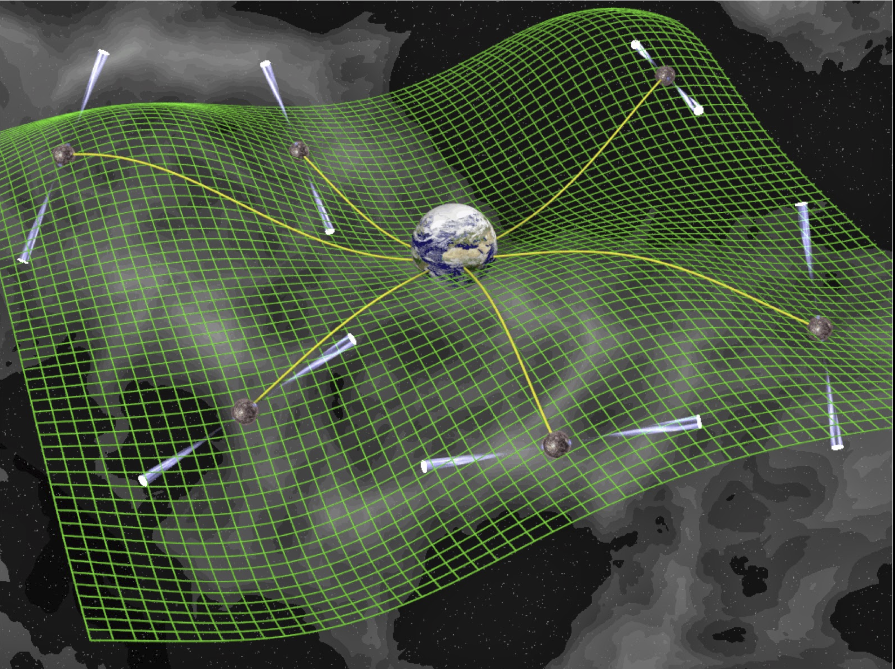
\includegraphics[width=0.85\textwidth]{pt11.png}
\caption[Pulsar timing]{Artist's conception shows the correlation of the signal from set of pulsars. Pulsar timing is using the residuals from each signals to obtains the TOAs which then can be used to detect the gravitational waves background. Image credit: David J. Champion }
\label{fig:pulsar timing}
\end{figure}


The project consists three individual projects as the following: 
\subsubsection*{European Pulsar Array (EPTA)}
This project consists of Jodrell Bank, Effelsberg, Westerbork and Nancay telescopes each 100-m diameter in Europe. Using these telescopes, the project is producing a high precision timing observation for more than 15 pulsars.

\subsubsection*{Parkes Pulsar Array (PPTA)}
Making use of Parkes radio telescope, 64-m in Australia, to observe 20 pulsars for one hour every two-three weeks. The telescope uses two receivers, 10cm-50cm and 20cm to perform the observation of one hour successively.

\subsubsection*{North American Nanohertz Observatory for Gravitational Waves (NANOGrav))}
Using Arecibo radio telescope, 300-m, and Green Bank telescope in the United States to carry out monthly observations for 24 pulsars.\\


\subsubsection*{International Pulsar Timing Array (IPTA)}
As the main aim of PTAs is to deliver a direct detection of low-frequency gravitational waves, the data from the three PTAs have combined in the so-called International Pulsar Timing Array (IPTA). see \citet{hobbs2010international}


































 
% Chapter Template

\chapter{Observations} % Main chapter title

\label{Chapter3} % Change X to a consecutive number; for referencing this chapter elsewhere, use \ref{ChapterX}

\lhead{Chapter 3. \emph{Observations}} % Change X to a consecutive number; this is for the header on each page - perhaps a shortened title

%----------------------------------------------------------------------------------------
%    SECTION 1
%----------------------------------------------------------------------------------------
\section{ Introduction}

In this chapter we giving the general over view about the observations used in the study as well as the instrument used to observe them.\\

We used observation from three International LOFAR stations, FR606, SE607 and DE60x. 

\section{LOw Frequency ARray (LOFAR)}
This section based on the full arterial about LOFAR (\citet{van2013lofar})\\

The Low Frequency Array, LOFAR is a unique radio telescope contains number of interferometric array of dipole antenna stations spread in Europe. LOFAR designed and developed by ASTRON, The Netherlands Institute for Radio Astronomy to operate in the low frequency regime of the radio wavelengths, between the 10 to 240 MHz which correspond to the wavelength from 30 to 1.2 m. Beside this, LOFAR also has large field of view, FoV which makes LOFAR an excellent instrument for many key sciences including pulsars and transients. For full details about LOFAR in pulsars and other key science (\citet{ stappers2011observing}). 

LOFAR's stations are mainly distributed in the Netherlands 40 stations and 9 international stations distributed within the partner Europeans countries, 6 in Germany, 3 in Poland and 1 each in France, England, Sweden, Ireland and Italy which joint the International Lofar Telescope, ITL early this year ( see \url{http://www.astron.nl/lofar-crosses-alps-italy-joins}) and Figure (\ref{fig:example1}). These stations are similar to the dishes in the typical radio telescope which can providing raw sensitivity, tracking the sources and collecting area. They classified as the following:

\subsection*{Core Stations}
A set of 24 stations located in the Netherlands with the radius of 
2km. The central region of this core, which contain 6 stations within the area of 320 m diameter is known as Superterp and it gives the shortest baselines for the whole array. All these stations has 96 Low Band Antenna (LBAs) and 48 High Band Antennas (HBAs).Figure (\ref{fig:example1}) showing the Superterp in the central circle of the Core, appear also number of the core stations around it.
\subsection*{Remote Stations}
These are 16 stations distributed approximately as a logarithmic spiral shape over the radius of 90 km. Both, Core and Remote stations distributed over radius of 180 km next to Exloo town in the northeastern Dutch province of Drenthe in the Netherlands.\\
Similar to the Core stations, the Remote stations also have 96 LBAs and 48 HBAs.

\subsection*{International Stations}
Currently, there are 8 functional international LOFAR stations distributed in Germany 5 station and one station of each of France, Sweden (Figure \ref{fig:example}) and England. Each station of these has 96 LBAs and 96 HBAs and 96 digital receiver units (RCUs) which gives total of 192 digital signal path during any single observation.





\begin{figure}[H]
    \centering
    \subfloat[label 1]{{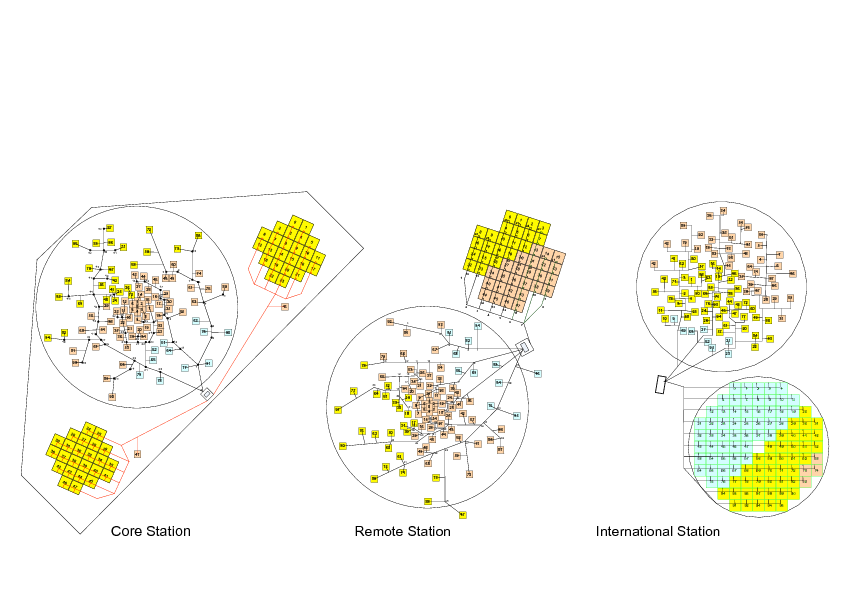
\includegraphics[width=11cm]{figures_LOFAR_stations_02.png} }}%
    \qquad
    \subfloat[label 2]{{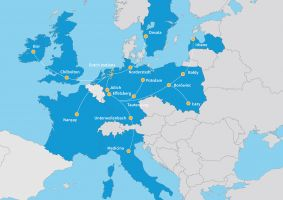
\includegraphics[width=10cm]{LOFAR_Map_2018_0_ITALY.jpg} }}%
    \caption{ (\citet{van2013lofar}) and \url{http://www.astron.nl/lofar-crosses-alps-italy-joins}}%
    \label{fig:example1}%
\end{figure}


\subsection*{High Band Antennas (HBAs)}

\subsection*{Low Band Antennas (LBAs)}



\begin{figure}[H]
    \centering
    \subfloat[Core Stations]{{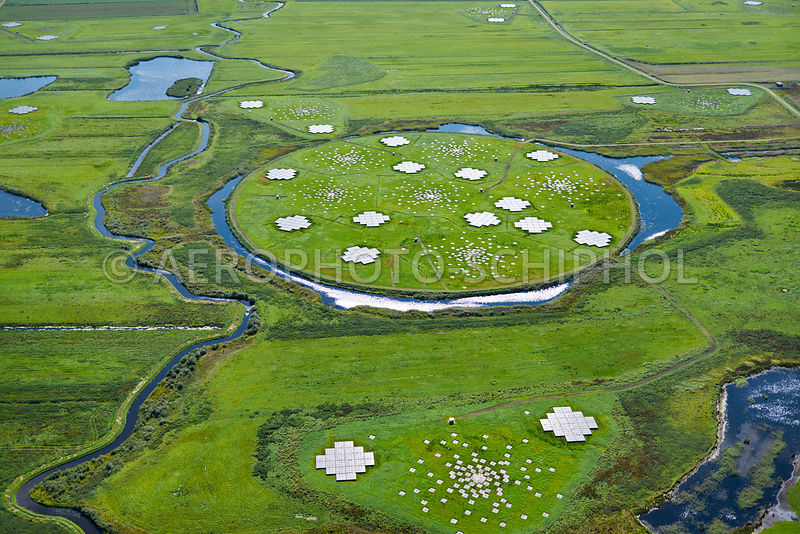
\includegraphics[width=10cm]{301620_xlarge.jpg} }}%
    \qquad
    \subfloat[Sewdish Station]{{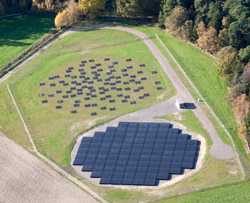
\includegraphics[width=10cm]{ONSALA.jpg} }}%
    \caption{ \citet{gunst2010lofar} and ONSALA (\url{https://www.aerophotostock.com/-/galleries/all/page/59} \url{http://lofar-se.org/})}%
    \label{fig:example}%
\end{figure}











\section{Observations}


\begin{tabular}{SSSSS}\toprule
    {Pulsar} & {B name} & {J name} & {DM ($cm^{-3}pc$)} & {LOFAR Station} \\ \midrule
    1  & {B0320+39}  & {J0141+6009} && FR606 \\
    2  & {B0320+39}  & {J0323+3944} && FR606 \\
    3  & {B1508+55}  & {J1509+5531} && FR606 \\
    4  & {B1737+13}  & {J1740+1311} && FR606 \\
    5  & {B1822-09}  & {J1825-0935} && FR606 \\
    6  & {B1931+24}  & {J1933+2421} && FR606 \\
    7  & {B2016+28}  & {J2018+2839} && FR606 \\
    8  & {B2111+46}  & {J2113+4644} && FR606 \\
    9  & {B2224+65}  & {J2225+6535} && FR606 \\
    10 & {B2310+42}  & {J2313+4253} && FR606 \\
    11 & {B0450+55}  & {J0454+5543} && FR606 \\
    12 & {B0540+23}  & {J0543+2329} && FR606 \\
    13 & {B0809+74}  & {J0814+7429} && FR606 \\
    14 & {B0834+06}  & {J0837+0610} && FR606 \\
    15 & {B0950+08}  & {J0953+0755} && FR606 \\
    16 & {B1133+16}  & {J1136+1551} && FR606 \\
    17 & {B1237+25}  & {J1239+2453} && FR606 \\
    18 & {B1540-06}  & {J1543-0620} && FR606 \\
    19 & {B1642-03}  & {J1645-0317} && FR606 \\
    20 &     {-}     & {J0613+3731} && FR606 \\
    21 & {B0329+54}  & {J0332+5434} && FR606 \\ \bottomrule
\end{tabular}














% Chapter Template

\chapter{Data Analysis and Results} % Main chapter title

\label{Chapter4} % Change X to a consecutive number; for referencing this chapter elsewhere, use \ref{ChapterX}

\lhead{Chapter 4. \emph{Data Analysis and Results}} % Change X to a consecutive number; this is for the header on each page - perhaps a shortened title

%----------------------------------------------------------------------------------------
%    SECTION 1
%---------------------------------------------------------------------------------------- 
% Chapter Template

\chapter{Discussion and Conclusions} % Main chapter title

\label{Chapter5} % Change X to a consecutive number; for referencing this chapter elsewhere, use \ref{ChapterX}

\lhead{Chapter 5. \emph{Discussion and Conclusions}} % Change X to a consecutive number; this is for the header on each page - perhaps a shortened title

%----------------------------------------------------------------------------------------
%    SECTION 1
%---------------------------------------------------------------------------------------- 
%\input{Chapters/Chapter6} 
%\input{Chapters/Chapter7} 

%----------------------------------------------------------------------------------------
%	THESIS CONTENT - APPENDICES
%----------------------------------------------------------------------------------------

\addtocontents{toc}{\vspace{2em}} % Add a gap in the Contents, for aesthetics

\appendix % Cue to tell LaTeX that the following 'chapters' are Appendices

% Include the appendices of the thesis as separate files from the Appendices folder
% Uncomment the lines as you write the Appendices

% Appendix A

\chapter{Appendix A} % Main appendix title

\label{AppendixA} % For referencing this appendix elsewhere, use \ref{AppendixA}

\lhead{Appendix A. \emph{A}} % This is for the header on each page - perhaps a shortened title

Write your Appendix content here.
%\input{Appendices/AppendixB}
%\input{Appendices/AppendixC}

\addtocontents{toc}{\vspace{2em}} % Add a gap in the Contents, for aesthetics

\backmatter

%----------------------------------------------------------------------------------------
%	BIBLIOGRAPHY
%----------------------------------------------------------------------------------------

\label{Bibliography}

\lhead{\emph{Bibliography}} % Change the page header to say "Bibliography"

\bibliographystyle{apalike} % Use the "apalike" BibTeX style for formatting the Bibliography

\bibliography{Bibliography} % The references (bibliography) information are stored in the file named "Bibliography.bib"

\end{document}